% ============================================================
% IEEE Conference Paper — HW5 ECG/HRV Multi-Paradigm Lab Study
% Template: IEEEtran conference (Overleaf compatible)
% ============================================================
\documentclass[conference]{IEEEtran}

% ---------- packages ----------
\usepackage{cite}
\usepackage{amsmath,amssymb}
\usepackage{graphicx}
\usepackage{grffile}          % robust filename handling (accented chars)
\usepackage{booktabs}
\usepackage{multirow}
\usepackage{siunitx}
\usepackage{textcomp}
\usepackage{url}
\usepackage{balance}
\usepackage{tabularx}

% BasicTeX often omits Adobe Courier (pcr/pcrr7t); use CM typewriter for \texttt.
\renewcommand{\ttdefault}{cmtt}

% ---------- figure path ----------
% Local LaTeX workspace loads canonical figure PDFs directly from outputs/figures/.
\graphicspath{{../outputs/figures/}}

% ---------- SI setup ----------
\sisetup{
  group-separator={,},
  detect-weight=true,
  detect-family=true
}

% ============================================================
\begin{document}

\title{HRV Interpretation Across Physiological Tasks Using Single-Lead ECG}

% --- authors ---
\author{
  \IEEEauthorblockN{Pei-En Wu}
  \IEEEauthorblockA{
    Department of Medicine and Department of Electrical Engineering
    \\
    National Yang Ming Chiao Tung University, Hsinchu, Taiwan\\
    Email: peienwu.ee13@nycu.edu.tw
  }
  \thanks{EEEC~1099 Biomedical Sensors --- HW5 Lab Report, April 2026.}
}

\maketitle

% ============================================================
\begin{abstract}
Heart rate variability (HRV) is widely used as a noninvasive marker of
autonomic regulation, but its interpretation depends strongly on
physiological context.
This single-participant lab study analyzed 14~single-lead ECG recordings
(500~Hz) across four task families specified by the assignment: postural
baseline (supine/sitting/standing), voluntary breath-hold (inspiratory
and expiratory, two trials each), walking with recovery, and a
self-designed variation of paced breathing at five rates (12, 9, 6, 5,
3~breaths/min).
Postural loading produced monotonic vagal withdrawal: mean HR rose from
54.0 to 79.7~bpm and RMSSD fell from 99.1 to 25.2~ms.
Inspiratory breath-hold produced larger HR excursions than expiratory
hold ($\Delta$HR up to +14.3 vs.\ +1.9~bpm).
Walking elevated HR to 83.0~bpm with rapid post-exercise recovery
($\tau = 6.8$~s), but motion artifacts limited fine-scale HRV
interpretation.
Paced breathing entrained the RR spectral peak with high fidelity
($R^{2} = 0.998$); LF/HF inflated from 0.22 to 17.47 while RMSSD
remained stable (47.7--64.9~ms), indicating spectral-band migration rather than
sympathovagal reversal.
We summarize the task-specific validity of standard HRV metrics in a
unified table and demonstrate that HRV indices must be interpreted
within the validity bounds imposed by the specific physiological task.
\end{abstract}

\begin{IEEEkeywords}
Heart rate variability, single-lead ECG, paced breathing, breath-hold,
spectral band migration, autonomic nervous system
\end{IEEEkeywords}

% ============================================================
\section{Introduction}
\label{sec:intro}

Heart rate variability quantifies beat-to-beat fluctuations in cardiac
cycle length, driven primarily by autonomic neural modulation of the
sinoatrial node~\cite{taskforce1996}.
Time-domain indices such as SDNN and RMSSD capture overall and
short-term variability, while frequency-domain decomposition into
low-frequency (LF: 0.04--0.15~Hz) and high-frequency (HF:
0.15--0.40~Hz) bands provides a spectral view of autonomic
oscillations~\cite{taskforce1996}.
The HF band primarily reflects respiratory sinus arrhythmia (RSA),
the phasic vagal modulation of heart rate coupled to the breathing
cycle~\cite{hirsch1981}.
HRV has become a standard noninvasive tool in cardiovascular research
and clinical risk stratification~\cite{berntson1997,shaffer2017}.

Despite its widespread adoption, HRV interpretation remains
context-dependent.
The LF/HF ratio, originally proposed as a sympathovagal balance
index~\cite{taskforce1996}, has been challenged on mechanistic
grounds: LF power reflects both sympathetic and parasympathetic
modulation, and the ratio becomes particularly unreliable when
respiratory frequency falls below the conventional 0.15~Hz boundary
separating LF from HF~\cite{billman2013,eckberg1997}.
Under such conditions, the dominant respiratory oscillation migrates
into the LF band, inflating LF/HF without a genuine shift in
autonomic balance.
This limitation is clinically relevant because slow-breathing
interventions are increasingly used in biofeedback
therapy~\cite{lehrer2014}.

This lab study addresses how the physiological meaning and validity of
common HRV metrics change across four task contexts: steady-state
posture, transient breath-hold, ambulatory motion, and externally paced
respiration.
We treat this as a within-subject lab investigation designed to expose
context-dependent interpretive limits of standard HRV indices.
We acquired 14~single-lead ECG recordings (500~Hz) from one participant
using a unified analysis pipeline spanning (1)~postural baseline,
(2)~voluntary breath-hold, (3)~ambulatory walking with recovery,
(4)~paced breathing at five rates.
This design eliminates inter-individual variability and allows direct
comparison of how the \emph{same} HRV indices behave under fundamentally
different physiological demands.

We formulated five hypotheses prior to data collection:
\begin{enumerate}
  \item[\textbf{H1}:]
    Progressive orthostatic loading (supine $\to$ sitting $\to$
    standing) produces monotonic increases in HR and decreases in
    vagal-linked indices (RMSSD, HF power).
  \item[\textbf{H2}:]
    Inspiratory breath-hold imposes a greater chronotropic challenge than
    expiratory breath-hold, consistent with altered thoracic mechanics
    and autonomic compensation.
  \item[\textbf{H3}:]
    Walking-phase fine-scale HRV (RMSSD) is contaminated by motion
    artifacts, whereas mean HR and post-exercise recovery kinetics remain
    interpretable.
  \item[\textbf{H4}:]
    Within the tested paced-breathing range (3--12~breaths/min), RR
    oscillation amplitude does not exhibit a classical resonance maximum
    centered at 6~breaths/min.
  \item[\textbf{H5}:]
    When breathing frequency falls below 0.15~Hz, the resulting LF/HF
    inflation reflects spectral-band migration, not sympathovagal shift,
    and therefore dissociates from RMSSD.
\end{enumerate}
Note that successful entrainment of the RR spectral peak by paced
breathing (verified by linear regression of measured vs.\ imposed
frequency) is treated as a manipulation check rather than a hypothesis,
since respiratory entrainment of the cardiac cycle is
well-established.

Our contributions are threefold.
First, we provide an end-to-end ECG analysis framework---from data
quality control and dual-path R-peak validation through
experiment-specific readouts to cross-experiment synthesis.
Second, we show that different tasks demand different interpretive
spaces: posture maps a steady-state autonomic set-point axis;
breath-hold and walking reveal transient challenge--recovery
trajectories; paced breathing modulates oscillation amplitude and
spectral location.
Third, we consolidate these observations into a task-specific HRV
metric validity summary (Table~\ref{tab:validity}), providing a
practical reference for interpreting HRV under each tested condition.

Table~\ref{tab:assignment_map} maps each assignment question to the
corresponding experiment, results section, and main-text figures.

\begin{table}[h]
\caption{Assignment Coverage Map (EEEC~1099 HW5)}
\label{tab:assignment_map}
\centering
\resizebox{\columnwidth}{!}{%
\begin{tabular}{@{}llll@{}}
\hline
Assignment Question & Experiment & Section & Main Figures \\
\hline
Q1: Postural baseline & E1 (A/B/C) & \ref{ssec:posture} &
  Fig.~\ref{fig:posture}--\ref{fig:poincare} \\
Q2: Transpulmonary effects & E2 (insp/exp) & \ref{ssec:breathhold} &
  Fig.~\ref{fig:breathhold}--\ref{fig:hf_collapse} \\
Q3: Ambulatory recording & E3 & \ref{ssec:walking} &
  Fig.~\ref{fig:walk_motion}--\ref{fig:walk_ecg_psd} \\
Q4: Self-designed variation & E4: paced breathing & \ref{ssec:paced} &
  Fig.~\ref{fig:e4a_tachograms}--\ref{fig:e4a_resp_resonance} \\
Cross-experiment synthesis & All & \ref{ssec:integration} &
  Fig.~\ref{fig:integration}, Table~\ref{tab:validity} \\
\hline
\end{tabular}}
\end{table}


% ============================================================
\section{Materials and Methods}
\label{sec:methods}

\subsection{Study Design and Protocol}
\label{ssec:protocol}

A single healthy male participant (age 22, no known cardiovascular
or respiratory conditions) was instrumented with a VitalSigns VS-ECG
single-lead chest-patch sensor sampling ECG at 500~Hz and triaxial
accelerometry at 25~Hz.
All 14~recordings were acquired in a single session on April~24,
2026, under quiet indoor conditions.
Because every recording came from the same acquisition chain and was
processed with a unified pipeline, between-condition differences
primarily reflect task-dependent physiology rather than
instrumentation changes.

The protocol comprised four experiment families
(Table~\ref{tab:protocol}):

\begin{enumerate}
\item \textbf{Postural baseline (E1).}
  After a 5-min rest, three consecutive 5-min recordings were obtained
  in supine (E1A), sitting (E1B), and standing (E1C) postures.
  The participant maintained relaxed spontaneous breathing throughout.

\item \textbf{Voluntary breath-hold (E2).}
  In a seated position, the participant performed two trials of
  maximum inspiratory breath-hold ($\sim$20~s each) followed by 40~s
  of recovery breathing, and two trials of maximum expiratory
  breath-hold with the same protocol.
  Inter-trial rest was provided until baseline HR was restored.

\item \textbf{Walking challenge (E3).}
  A 180-s continuous recording was segmented into 60~s seated
  baseline, 60~s walking at self-selected pace, and 60~s seated
  recovery.

\item \textbf{Paced breathing (E4).}
  \emph{Self-designed variation (Assignment Q4).}
  This experiment served as the self-designed variation required by the
  assignment, formulated to test hypotheses \textbf{H4} and \textbf{H5}
  regarding the resonance question and LF/HF spectral-band migration
  under slow respiration.
  Five conditions were recorded in a seated position at fixed
  breathing rates of 12, 9, 6, 5, and 3~breaths/min, guided by a
  metronome.
  Each condition lasted approximately 4~min; the 3-breaths/min
  condition was extended to $\sim$5~min to ensure $\geq$14 complete
  breathing cycles.
  \emph{Limitation}: the five rates were presented in fixed
  descending order (12$\to$3), so progressive relaxation, training,
  or fatigue effects cannot be fully separated from the
  breathing-rate manipulation.

\end{enumerate}

\begin{table}[!t]
\centering
\caption{Experimental Protocol Summary}
\label{tab:protocol}
\footnotesize
\begin{tabular}{@{}llcc@{}}
\toprule
Family & Condition & Duration (s) & Posture \\
\midrule
E1 Postural & E1A Supine    & 300 & Supine \\
             & E1B Sitting   & 300 & Sitting \\
             & E1C Standing  & 300 & Standing \\
\midrule
E2 Breath-hold & Insp.\ $\times 2$ & 120 each & Sitting \\
               & Exp.\ $\times 2$  & 120 each & Sitting \\
\midrule
E3 Walking & Rest/Walk/Recovery & 180 & Sitting/Walk \\
\midrule
E4 Paced & 12, 9, 6, 5, 3/min & 220--280 & Sitting \\
\bottomrule
\end{tabular}
\end{table}


\subsection{Signal Processing}
\label{ssec:sigproc}

All processing was performed in Python~3.10 using a unified pipeline
(\texttt{src/pipeline.py}).
Raw ECG was corrected for baseline drift with a two-stage median
filter (200~ms and 600~ms kernel widths), then filtered with a 50~Hz
second-order IIR notch ($Q = 30$) to suppress power-line interference,
followed by a 0.5--40~Hz fourth-order Butterworth bandpass
(zero-phase via \texttt{sosfiltfilt})~\cite{virtanen2020}.

R-peak detection followed two parallel paths to ensure pipeline
robustness (Fig.~\ref{fig:pipeline_overview}):
\begin{itemize}
\item \emph{Teaching path}: a Pan--Tompkins-style detector implemented
  in SciPy~\cite{pan1985}, providing a transparent, interpretable
  reference.
\item \emph{Reference path}: NeuroKit2 \texttt{ecg\_peaks} with
  Kubios-style artifact correction~\cite{makowski2021}, serving as
  the primary path for reported results due to its superior handling
  of short transient segments.
\end{itemize}
Pipeline validation on a 5-min steady-state recording (E1A)
confirmed $\geq$99.5\% peak-count agreement between paths, with
mean RR difference $<$1.0~ms and RMSSD difference $<$2.7~ms.

\begin{figure}[!t]
\centering
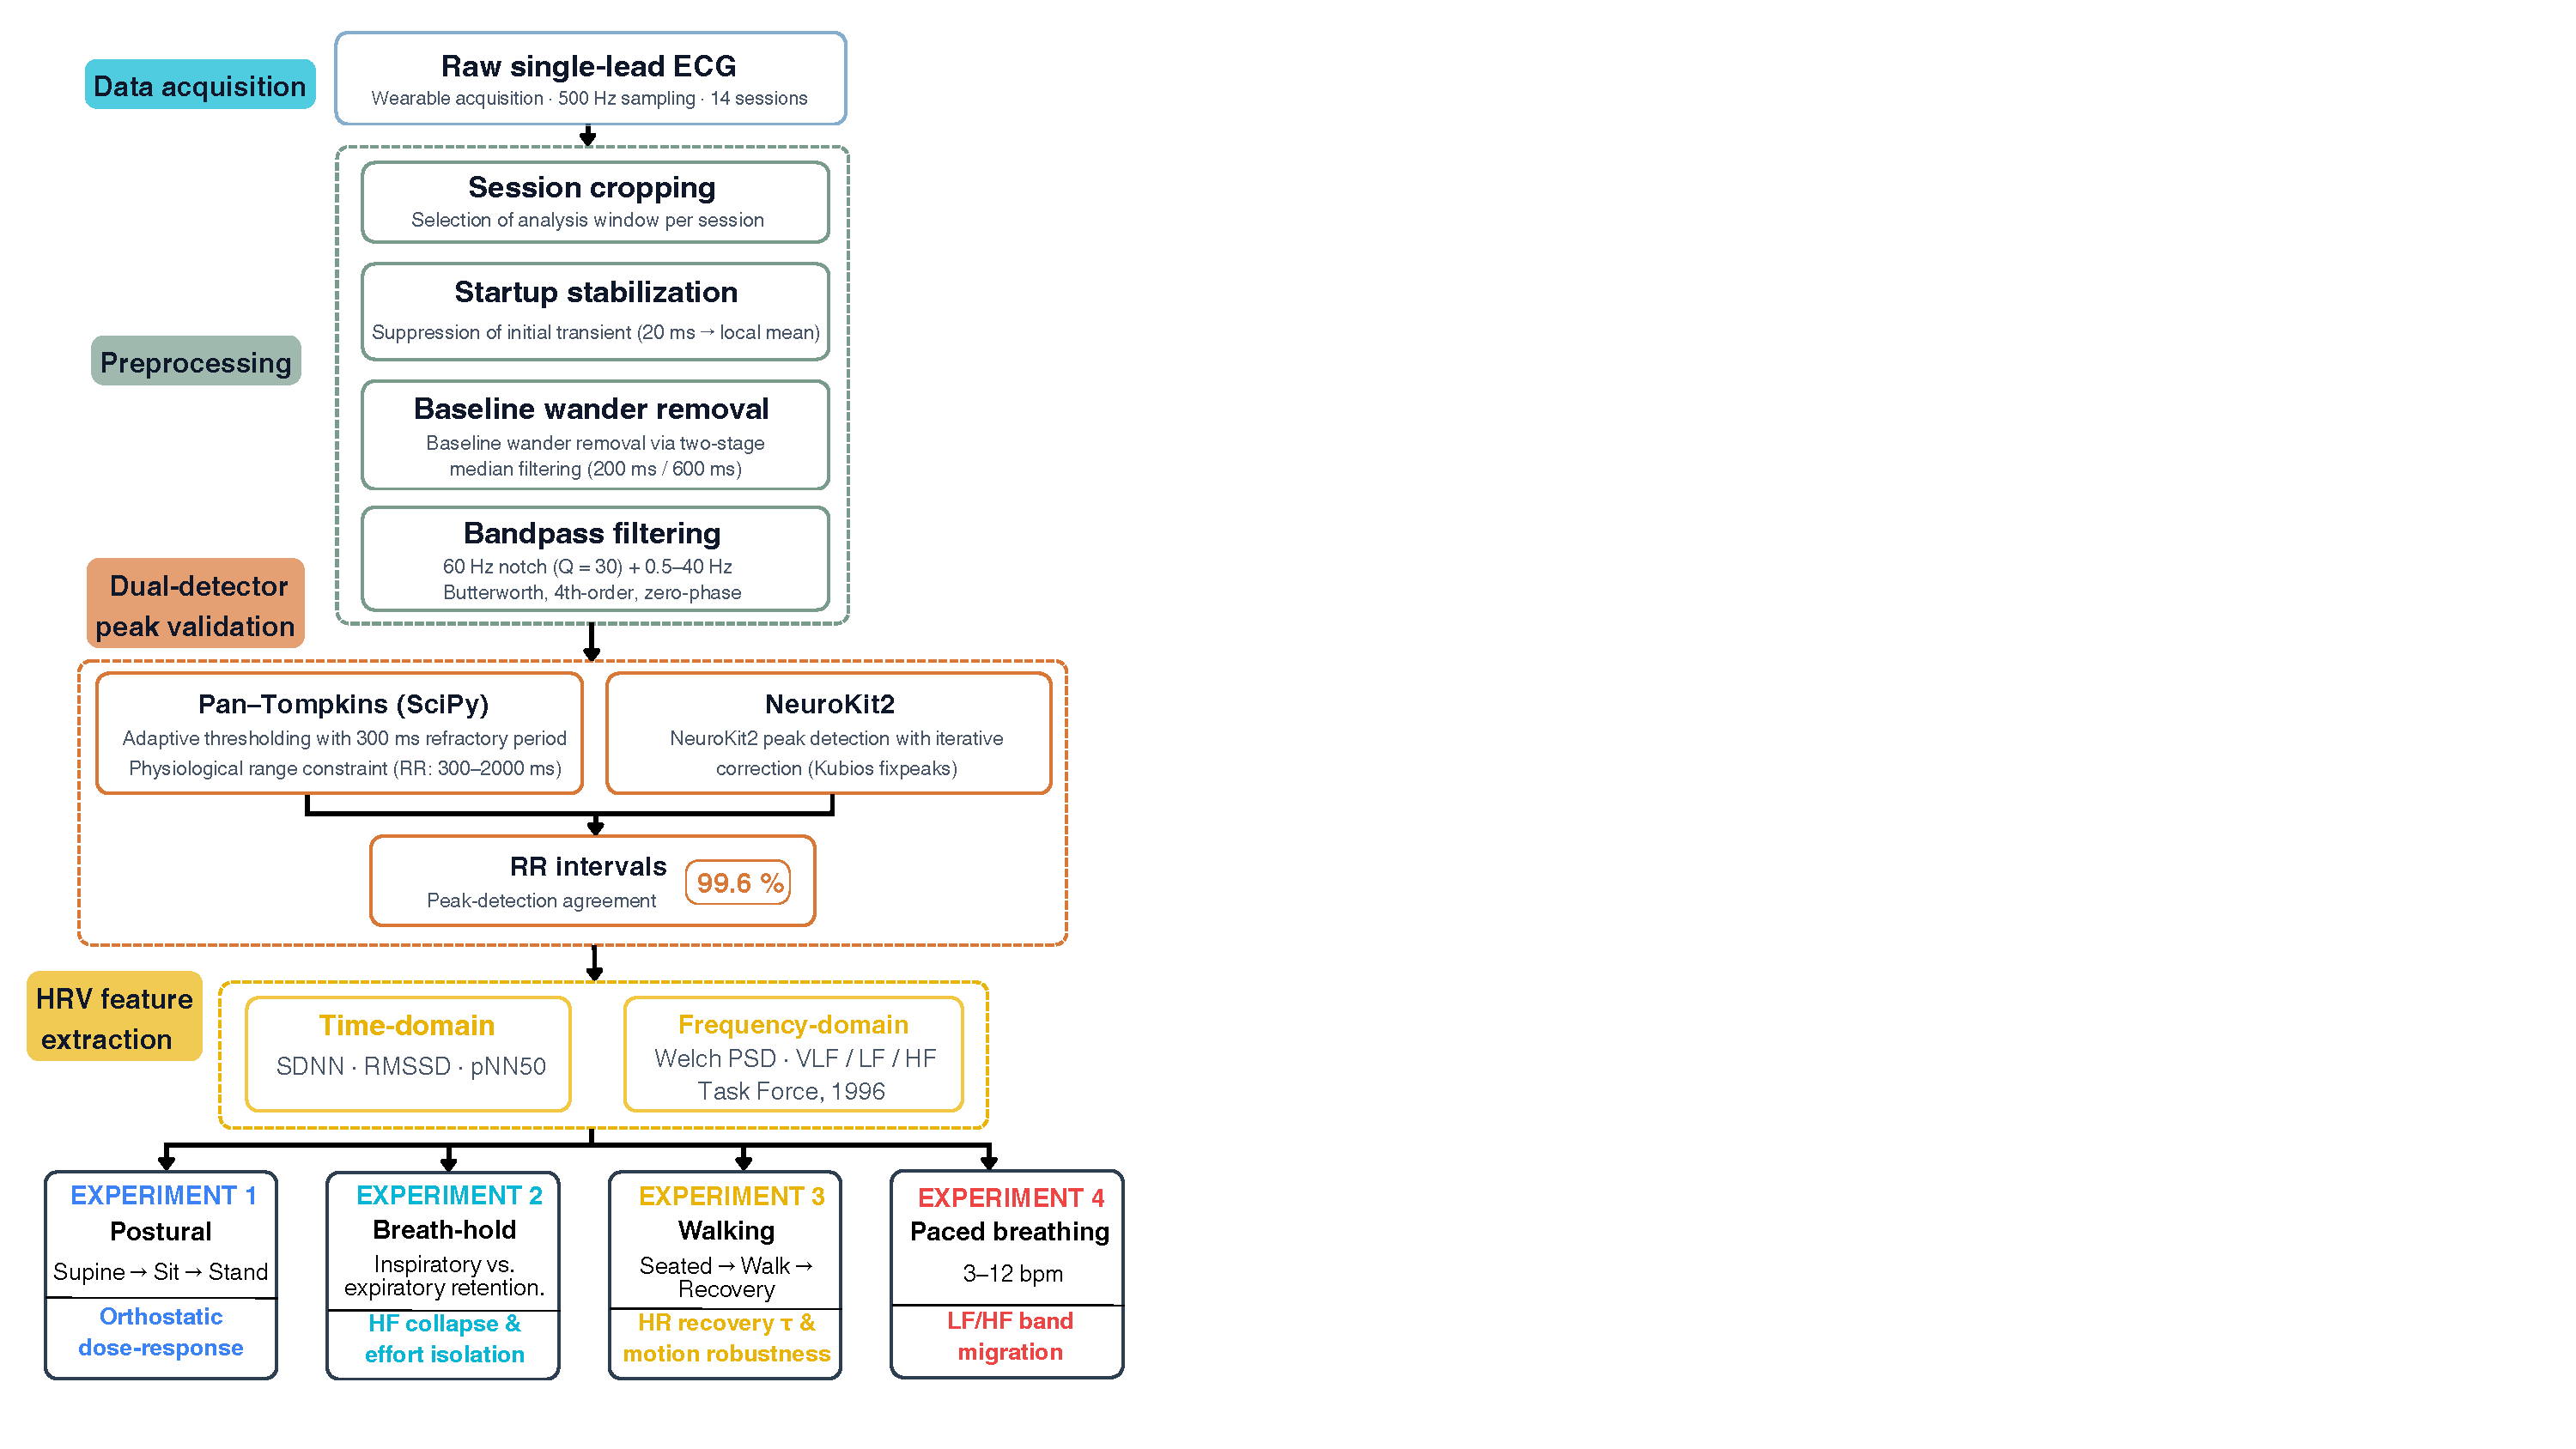
\includegraphics[width=\columnwidth]{nb01_fig01_pipeline_overview.pdf}
\caption{End-to-end ECG analysis pipeline. Raw ECG is preprocessed
with baseline correction and bandpass filtering, then processed
through dual-path R-peak detection (SciPy teaching path and
NeuroKit2 reference path) before experiment-specific HRV analysis.}
\label{fig:pipeline_overview}
\end{figure}


\subsection{HRV Analysis}
\label{ssec:hrv}

HRV indices were computed following the Task Force
standards~\cite{taskforce1996}.
RR intervals outside the 300--2000~ms physiological range were
rejected.
For steady-state conditions (E1, E4), the full analysis window
($\geq$220~s) was used.
Window-length sensitivity on the E1A supine recording (Appendix,
Fig.~\ref{fig:app_duration}) showed that sliding-window coefficient of
variation fell below 10\% for SDNN and below 5\% for HF once segment
duration reached $\sim$180~s, whereas 30--60~s windows exhibited much
higher variability; this supports our use of full multi-minute
windows---including 5-min postural baselines (E1) and the
$\geq$220~s steady-state segments for paced breathing---for stable
time- and frequency-domain HRV estimation.

\textbf{Time domain.}
Mean HR, SDNN, RMSSD, and pNN50 were computed from the edited
RR series.

\textbf{Frequency domain.}
The RR series was linearly detrended and resampled at 4~Hz via cubic
interpolation~\cite{taskforce1996}.
Power spectral density (PSD) was estimated using Welch's method
(256-point Hann window, 50\% overlap).
Band powers were integrated over the Task Force frequency ranges:
VLF (0.003--0.04~Hz), LF (0.04--0.15~Hz), and HF (0.15--0.40~Hz).
Normalized units were computed as
$\text{LF}_\text{n.u.} = \text{LF} / (\text{TP} - \text{VLF})
\times 100$.

\textbf{Transient conditions (E2, E3).}
Because individual phases (hold, walk, recovery) lasted only
20--60~s, standard frequency-domain HRV was not computed
per-phase~\cite{taskforce1996}.
Instead, we reported regime-based mean~HR, RMSSD, HR~range, and
HR~slope.
For E2, frequency-domain HRV indices (HF power, LF/HF) were
computed per trial using the same Welch method, and spectral
comparison was performed against the E1B seated anchor.

\textbf{Walking recovery kinetics.}
Post-walking HR recovery was fitted to a single-exponential decay
model:
\begin{equation}
  \text{HR}(t) = \text{HR}_{\infty}
  + (\text{HR}_{0} - \text{HR}_{\infty})\,
    e^{-t/\tau},
\label{eq:recovery}
\end{equation}
using nonlinear least-squares (\texttt{scipy.optimize.curve\_fit})
over the 60-s post-walking recovery window.

\textbf{Motion contamination assessment.}
Walking-phase motion contamination was evaluated using two
complementary metrics.
First, Pearson correlation between absolute successive RR
differences ($|\Delta\text{RR}|$) and accelerometer vector magnitude
was computed during the walking segment ($r = 0.26$).
Second, magnitude-squared coherence ($C_{xy}$) between the walking
ECG and accelerometer-derived motion magnitude was estimated to test
whether a stable, phase-locked step-frequency component contaminated
the cardiac signal.
We acknowledge that fine-scale spectral coherence is a stronger
contamination indicator than amplitude correlation and discuss the
joint interpretation in Section~\ref{ssec:walking}.

\textbf{Paced-breathing frequency tracking.}
The dominant RR spectral peak was identified for each paced-breathing
condition and compared against the imposed breathing frequency using
ordinary least-squares regression.
Slope, intercept, $R^{2}$, and 95\% confidence intervals were
reported; the null hypotheses slope~$=1$ and intercept~$=0$ were
tested.

\textbf{Respiratory-centered spectral analysis.}
To assess resonance independently of fixed LF/HF band boundaries,
respiratory-centered RR spectral power was computed by integrating
the Welch PSD within a narrow window around each imposed breathing
frequency.
The primary integration window was $\pm$0.015~Hz; sensitivity
analyses were performed with $\pm$0.010~Hz and $\pm$0.020~Hz
windows.
This approach avoids the confound that arises when breathing
frequency crosses the 0.15~Hz LF/HF boundary, because the
integration window tracks the respiratory peak rather than relying
on fixed spectral bands.
RR oscillation amplitude was additionally quantified as the
distribution-based p95--p5 range, which is robust against
cycle-level detection instability in the absence of a direct
respiratory belt signal.


% ============================================================
\section{Results}
\label{sec:results}

\subsection{Postural Baseline Established a Coherent
Autonomic Reference Axis (\textbf{H1 Supported})}
\label{ssec:posture}

Progressive orthostatic loading produced the expected monotonic
autonomic redistribution (Table~\ref{tab:posture},
Fig.~\ref{fig:posture}--\ref{fig:poincare}).
From supine to standing, mean HR increased from 54.0 to 79.7~bpm,
RMSSD decreased from 99.1 to 25.2~ms, HF power dropped from 3252.8
to 310.7~ms$^{2}$, and LF/HF rose from 0.28 to 1.44.
These changes are consistent with progressive vagal withdrawal under
orthostatic stress~\cite{taskforce1996} and support \textbf{H1}.

The ECG power spectral density (Fig.~\ref{fig:ecg_psd}) further
reveals the heartbeat fundamental frequency ($f_{0}$) and its
harmonics ($2f_{0}$, $3f_{0}$), along with respiratory modulation
visible as a low-frequency spectral peak, across all three postures.

Poincar\'e return maps (Fig.~\ref{fig:poincare}) provide a
complementary nonlinear view of beat-to-beat variability: the
scatter cloud contracts progressively from supine to standing,
consistent with the reduction in short-term vagal modulation
measured by RMSSD.

The sitting baseline (E1B) was subsequently used as the
posture-matched anchor for the seated breath-hold and walking
experiments, ensuring that between-experiment spectral comparisons
are not confounded by postural differences.

In direct response to the assignment questions: (1)~the main
heartbeat frequency ($f_{0}$) and its harmonics ($2f_{0}$,
$3f_{0}$) are clearly visible in the ECG PSD across all three
postures (Fig.~\ref{fig:ecg_psd}); (2)~the breathing frequency is
identifiable as a low-frequency modulation peak; (3)~successive
heartbeat interval differences (Fig.~\ref{fig:posture}) show clearly
larger amplitude in supine than in standing, visualizing the postural
reduction in vagal modulation.

\begin{table}[!t]
\centering
\caption{Postural Baseline HRV Summary}
\label{tab:posture}
\footnotesize
\begin{tabular}{@{}lccc@{}}
\toprule
Metric & Supine & Sitting & Standing \\
\midrule
Mean HR (bpm)           & 54.0  & 56.1  & 79.7 \\
SDNN (ms)               & 81.5  & 56.6  & 41.8 \\
RMSSD (ms)              & 99.1  & 61.1  & 25.2 \\
pNN50 (\%)              & 62.2  & 43.5  & 2.8 \\
Total Power (ms$^{2}$)  & 4321.9 & 2016.6 & 1047.8 \\
LF (ms$^{2}$)           & 907.1 & 601.3 & 448.0 \\
HF (ms$^{2}$)           & 3252.8 & 1122.6 & 310.7 \\
LF n.u.\ (\%)           & 21.8  & 34.9  & 59.0 \\
HF n.u.\ (\%)           & 78.2  & 65.1  & 41.0 \\
LF/HF                   & 0.28  & 0.54  & 1.44 \\
\bottomrule
\end{tabular}
\end{table}

\begin{figure}[!t]
\centering
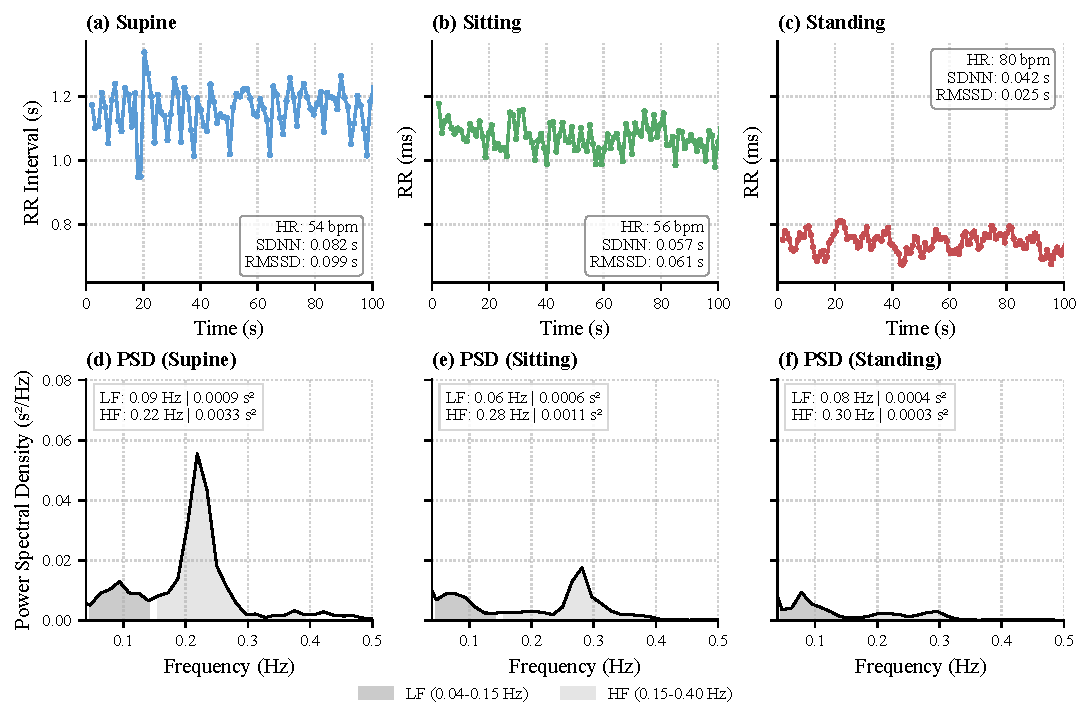
\includegraphics[width=\columnwidth]{nb02_fig03_rr_psd_postural.pdf}
\caption{Postural RR tachograms (top row) and RR interval power
spectral density (bottom row) for supine, sitting, and standing
conditions.  RR intervals are displayed in seconds.  Beat-to-beat
successive differences are visible as the point-to-point variations
in the tachogram, showing clearly larger amplitude in supine than in
standing.  Shaded regions indicate LF (orange) and HF (teal) bands
per Task Force definitions~\cite{taskforce1996}.  HF power decreases
monotonically from supine to standing, consistent with progressive
vagal withdrawal.}
\label{fig:posture}
\end{figure}

\begin{figure}[!t]
\centering
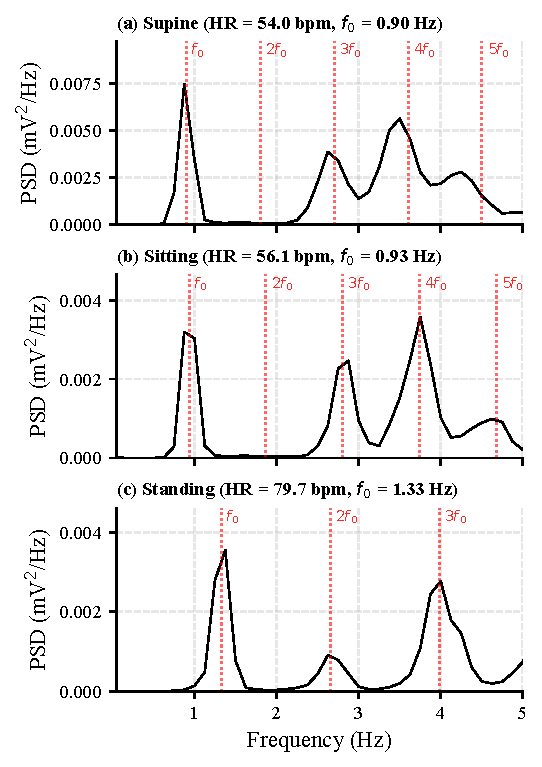
\includegraphics[width=\columnwidth]{nb02_fig02_ecg_psd_harmonics.pdf}
\caption{ECG power spectral density (0.05--5~Hz) reveals heartbeat
fundamental frequency, harmonics, and respiratory modulation across
postures.  The fundamental frequency $f_{0}$ shifts from
$\sim$0.90~Hz (supine, HR\,=\,54.0~bpm) to $\sim$1.33~Hz (standing,
HR\,=\,79.7~bpm).  Harmonic peaks at $2f_{0}$ and $3f_{0}$ are
clearly visible, consistent with the QRS complex morphology.  The
breathing frequency is identifiable as a low-frequency modulation
peak in supine recordings.  Direct response to assignment Q1:
heartbeat frequency, harmonics, and breathing frequency are all
observable.}
\label{fig:ecg_psd}
\end{figure}

% NOTE: If the accented filename causes compilation issues, rename the
% Exported as nb02_fig05_poincare_plot.pdf (ASCII filename).
\begin{figure}[!t]
\centering
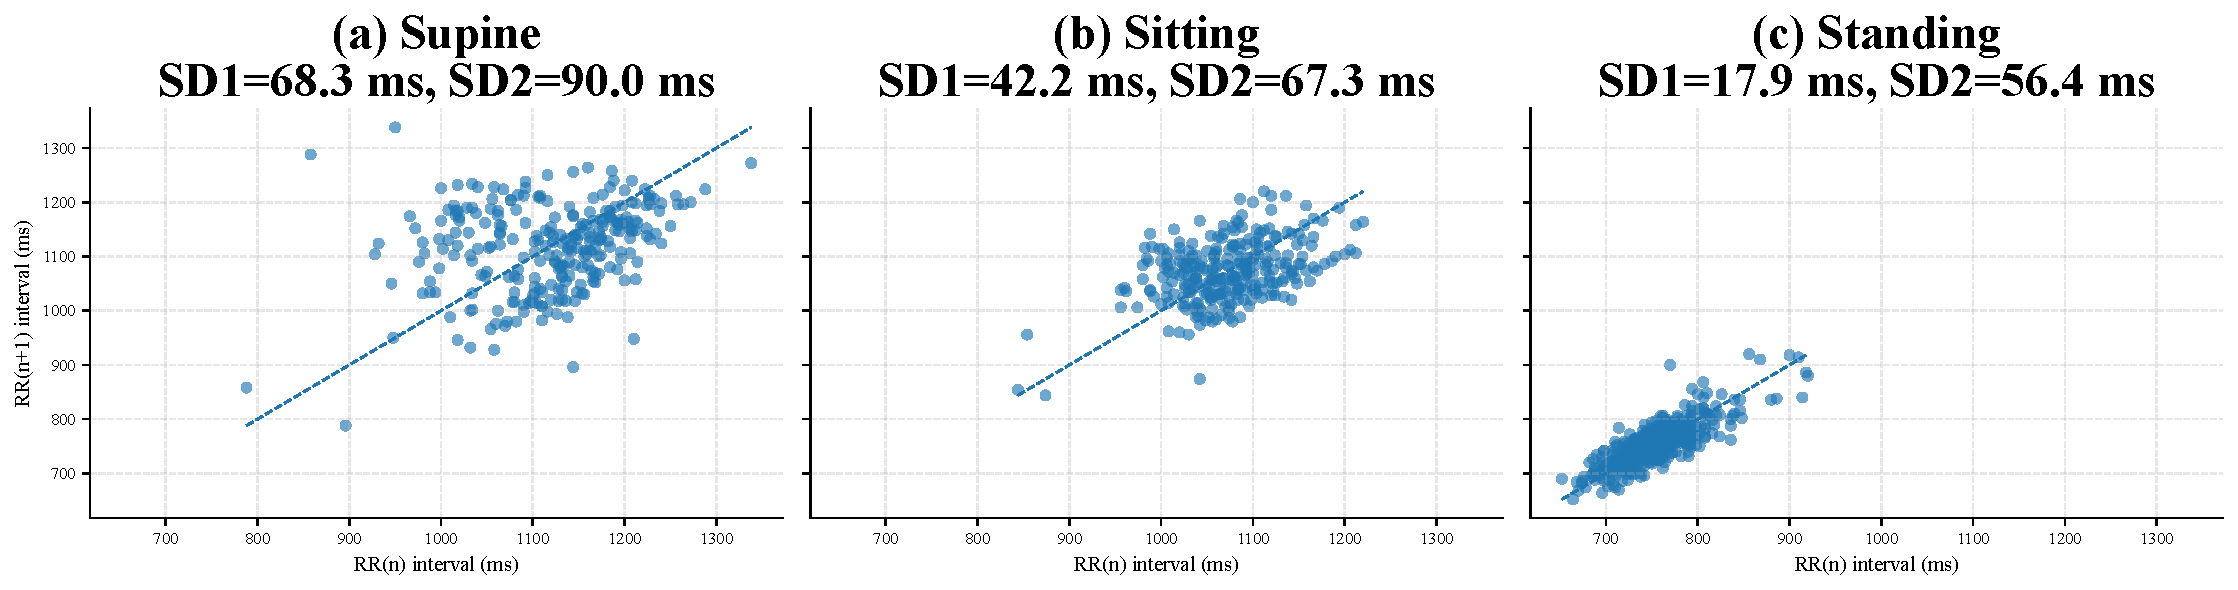
\includegraphics[width=\columnwidth]{nb02_fig05_poincare_plot.pdf}
\caption{Poincar\'e return maps ($\text{RR}_{n+1}$ vs.\
$\text{RR}_{n}$) for supine, sitting, and standing conditions.  The
scatter cloud contracts progressively from supine to standing,
reflecting reduced short-term vagal modulation consistent with the
RMSSD decrease shown in Table~\ref{tab:posture}.}
\label{fig:poincare}
\end{figure}


% ------ Breath-Hold ------
\subsection{Breath-Hold Effects Were Modulated by
Respiratory Mode and Effort (\textbf{H2 Supported})}
\label{ssec:breathhold}

Inspiratory breath-hold produced substantially larger chronotropic
responses than expiratory hold (Table~\ref{tab:breathhold},
Fig.~\ref{fig:breathhold}).
Across two inspiratory trials, mean hold-phase HR rose to 66.9 and
73.5~bpm ($\Delta$HR = +4.0 and +14.3~bpm relative to pre-hold
baseline), whereas expiratory hold-phase HR remained near baseline
(57.8 and 60.8~bpm; $\Delta$HR = $-$0.9 and +1.9~bpm).
The large inter-trial variability in the inspiratory condition
(CV of pre-hold HR: 4.3\% vs.\ 0.2\% for expiratory) suggests that
conscious effort and volitional strategy---not merely the absence
of respiration---shape the breath-hold response, supporting
\textbf{H2}.

Spectral comparison against the E1B seated anchor reinforced this
asymmetry (Fig.~\ref{fig:hf_collapse}).
To isolate the pure respiratory-cessation effect from volitional
effort, only the relaxed trial (Trial~2) was used for spectral
quantification; the effort confound is addressed separately in
Fig.~\ref{fig:breathhold}.
Inspiratory hold HF power collapsed to 39.1~ms$^{2}$ (a 28.7-fold
reduction from the anchor value of 1123~ms$^{2}$; $-$96.5\%),
whereas expiratory hold HF fell to 230.9~ms$^{2}$
(4.9-fold; $-$79.4\%).
Both conditions recovered to near-anchor levels within the 50~s
post-hold window (inspiratory: 1207~ms$^{2}$, $\times$1.07;
expiratory: 1213~ms$^{2}$, $\times$1.08), confirming that the
HF suppression is a transient, fully reversible perturbation
driven by apnoea itself rather than lingering sympathetic activation.

\begin{table}[!t]
\centering
\caption{Breath-Hold Trial-Level Metrics.  Trial~1 = effortful hold;
  Trial~2 = relaxed hold (see Fig.~\ref{fig:breathhold}).
  HF power is reported for the relaxed trial only, because the
  opposing HR-slope directions between trials ($-$0.19 vs.\ +0.18~bpm/s
  for inspiratory) violate the stationarity assumption required for
  ensemble spectral averaging.}
\label{tab:breathhold}
\footnotesize
\begin{tabular}{@{}lcccc@{}}
\toprule
 & \multicolumn{2}{c}{Inspiratory} & \multicolumn{2}{c}{Expiratory} \\
\cmidrule(lr){2-3}\cmidrule(lr){4-5}
Metric & Trial~1 & Trial~2 & Trial~1 & Trial~2 \\
\midrule
Pre-hold HR (bpm)   & 62.9 & 59.2 & 58.8 & 58.9 \\
Hold mean HR (bpm)  & 66.9 & 73.5 & 57.8 & 60.8 \\
$\Delta$HR (bpm)    & +4.0 & +14.3 & $-$0.9 & +1.9 \\
HR slope (bpm/s)    & $-$0.19 & +0.18 & $-$0.10 & $-$0.11 \\
Recovery HR (bpm)   & 79.2 & 64.8 & 59.2 & 57.4 \\
\midrule
\multicolumn{5}{@{}l}{\emph{HF power, relaxed trial only
  (vs.\ E1B anchor, 1123~ms$^{2}$):}} \\
Hold HF (ms$^{2}$) & — & 39.1 & — & 230.9 \\
Recovery HF (ms$^{2}$) & — & 1207 & — & 1213 \\
\bottomrule
\end{tabular}
\end{table}

\begin{figure}[!t]
\centering
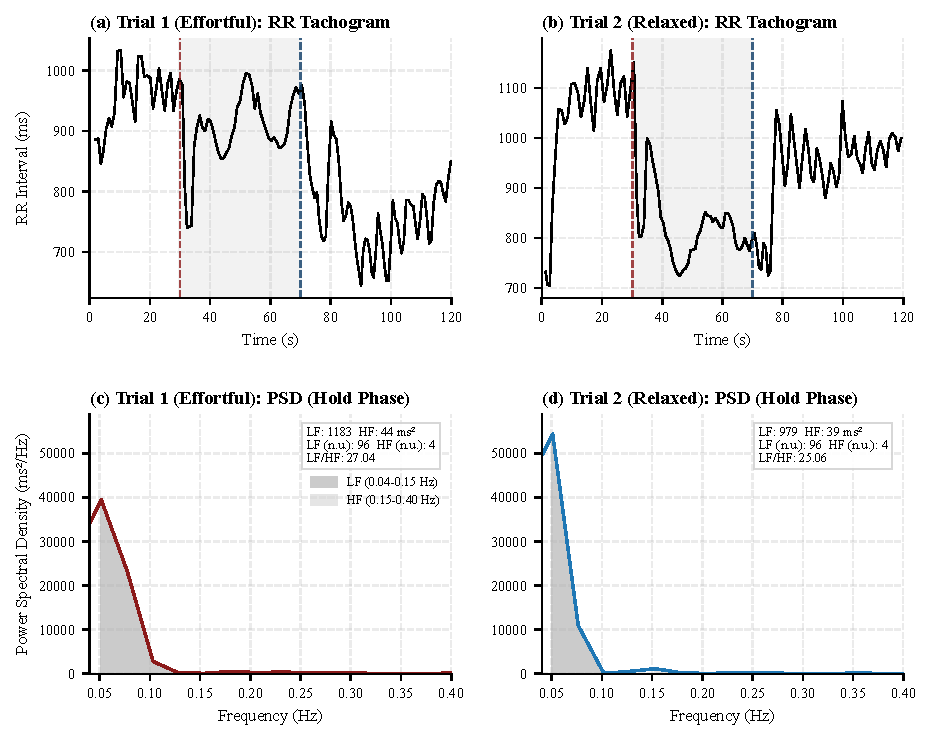
\includegraphics[width=\columnwidth]{nb03_fig02_e2_effort_vs_relaxed.pdf}
\caption{Breath-hold effort comparison.  Inspiratory hold (top panels)
produces larger HR excursions and more variable response shapes than
expiratory hold (bottom panels), indicating that conscious effort
modulates the physiological response beyond the respiratory
perturbation alone.}
\label{fig:breathhold}
\end{figure}

\begin{figure}[!t]
\centering
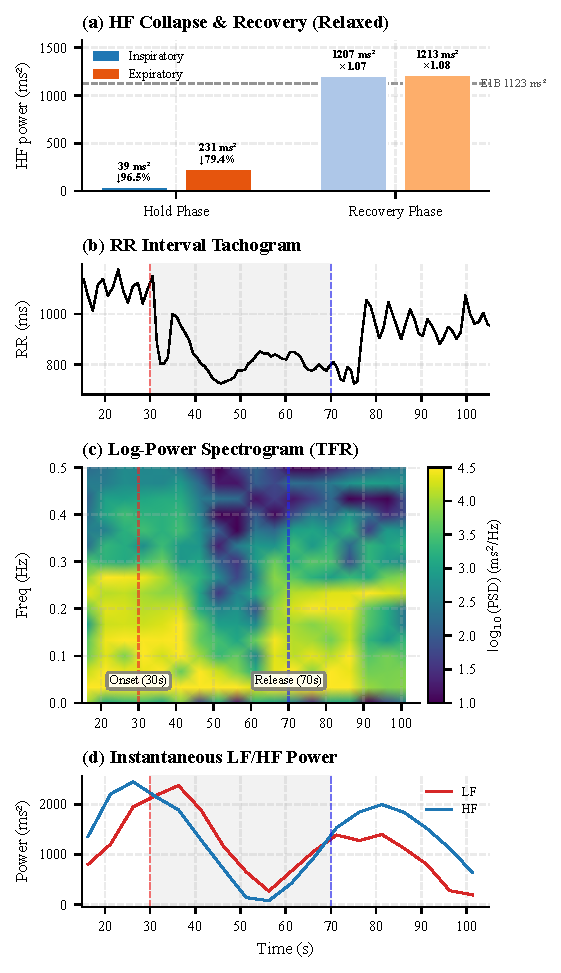
\includegraphics[width=\columnwidth]{nb03_fig01_e2_hf_collapse.pdf}
\caption{Breath-hold spectral dynamics (relaxed trial only).
(a)~HF power collapses during hold relative to the E1B seated
anchor (1123~ms$^{2}$): inspiratory hold shows a 28.7-fold
reduction ($-$96.5\%) versus a 4.9-fold reduction ($-$79.4\%)
for expiratory hold.  Both conditions recover to near-anchor
levels ($\times$1.07--1.08), indicating a fully reversible
vagal perturbation.
(b)--(d)~Representative inspiratory-relaxed trial showing
the RR tachogram, time--frequency spectrogram, and
instantaneous LF/HF power trajectories.}
\label{fig:hf_collapse}
\end{figure}


% ------ Walking ------
\subsection{Walking Produced Cardiovascular Load
but Required a Motion-Validity Framework (\textbf{H3 Supported})}
\label{ssec:walking}

The walking challenge produced an acute cardiovascular response
consistent with mild exercise (Table~\ref{tab:walking},
Figs.~\ref{fig:walk_motion},~\ref{fig:recovery_tau}).
Mean HR rose from 60.8~bpm (seated) to 83.0~bpm (walking) and
returned to 70.3~bpm during recovery, with a fitted exponential
time constant $\tau = 6.8$~s (Eq.~\ref{eq:recovery}).
This rapid recovery is consistent with parasympathetic reactivation
following low-intensity exercise~\cite{shaffer2017}.

However, walking-phase RMSSD (41.1~ms) should not be directly
compared with resting RMSSD because walking introduces
motion artifacts through multiple non-linear pathways---electrode-skin
impedance fluctuations, trunk EMG, and cable sway---that
cause random R-peak fiducial-point shifts and artificially inflate
beat-to-beat variability indices.
The raw walking ECG confirmed visible waveform degradation
(Fig.~\ref{fig:app_ecg_snapshots} in Appendix), and the walking-segment
ECG spectrum showed elevated broadband energy in the 1--3~Hz
locomotor band (Fig.~\ref{fig:walk_ecg_psd}).
Critically, the accelerometer-derived step frequency
(1.46~Hz) fell within 6\% of the walking heart-rate fundamental
($f_0 = 1.38$~Hz at 83~bpm), creating a spectral overlap that
precludes reliable separation of cardiac and locomotor components
by linear filtering alone.

We computed magnitude-squared coherence to test for phase-locked,
linear coupling between locomotor mechanics and the cardiac signal.
Coherence was low both at the step peak ($C_{xy} = 0.04$) and across
the 1--3~Hz cadence band (mean $C_{xy} = 0.06$, max~0.20), ruling out a
stable linear contamination pathway; Pearson correlation between
$|\Delta\text{RR}|$ and accelerometer magnitude was likewise weak
($r = 0.26$).
Low coherence does not, however, exclude non-linear artifacts such as
broadband baseline wander or stochastic fiducial-point jitter.
Combined with the cadence-proximate spectral energy in 1--3~Hz
(Fig.~\ref{fig:walk_ecg_psd}), we therefore flag walking-phase
fine-scale HRV as motion-limited.

In summary, mean HR and recovery kinetics---which depend on
slow trends robust to fiducial jitter---remain physiologically
interpretable, while fine-scale HRV indices such as RMSSD are
motion-limited.
The walking-phase HRV was accordingly flagged as
\textbf{unreliable~(motion)} in the summary table, supporting
\textbf{H3}.

In direct response to the assignment questions: (1)~motion
interference is observable in the walking-phase RR series and ECG
PSD, manifesting as elevated spectral energy in the 1--3~Hz band
coincident with the walking cadence identified independently from the
accelerometer (Fig.~\ref{fig:walk_ecg_psd},
Fig.~\ref{fig:walk_motion}); (2)~the post-walking rest segment
showed progressive lengthening of RR intervals with
$\tau = 6.8$~s, consistent with parasympathetic reactivation
following low-intensity exercise.

\begin{table}[!t]
\centering
\caption{Walking Challenge Segment Metrics}
\label{tab:walking}
\footnotesize
\begin{tabular}{@{}lcccc@{}}
\toprule
Segment & HR (bpm) & RMSSD (ms) & HR slope & Note \\
\midrule
Seated    & 60.8 & 54.4 & $-$0.06 & \\
Walking   & 83.0 & 41.1 & $-$0.12 & Motion$^\dagger$ \\
Recovery  & 70.3 & 46.9 & $-$0.13 & $\tau = 6.8$~s \\
\midrule
E1B anchor & 56.1 & 61.1 & --- & Seated ref. \\
\bottomrule
\multicolumn{5}{@{}l}{\footnotesize $^\dagger$Walking-phase HRV
  is motion-contaminated; interpret with caution.}
\end{tabular}
\end{table}

\begin{figure}[!t]
\centering
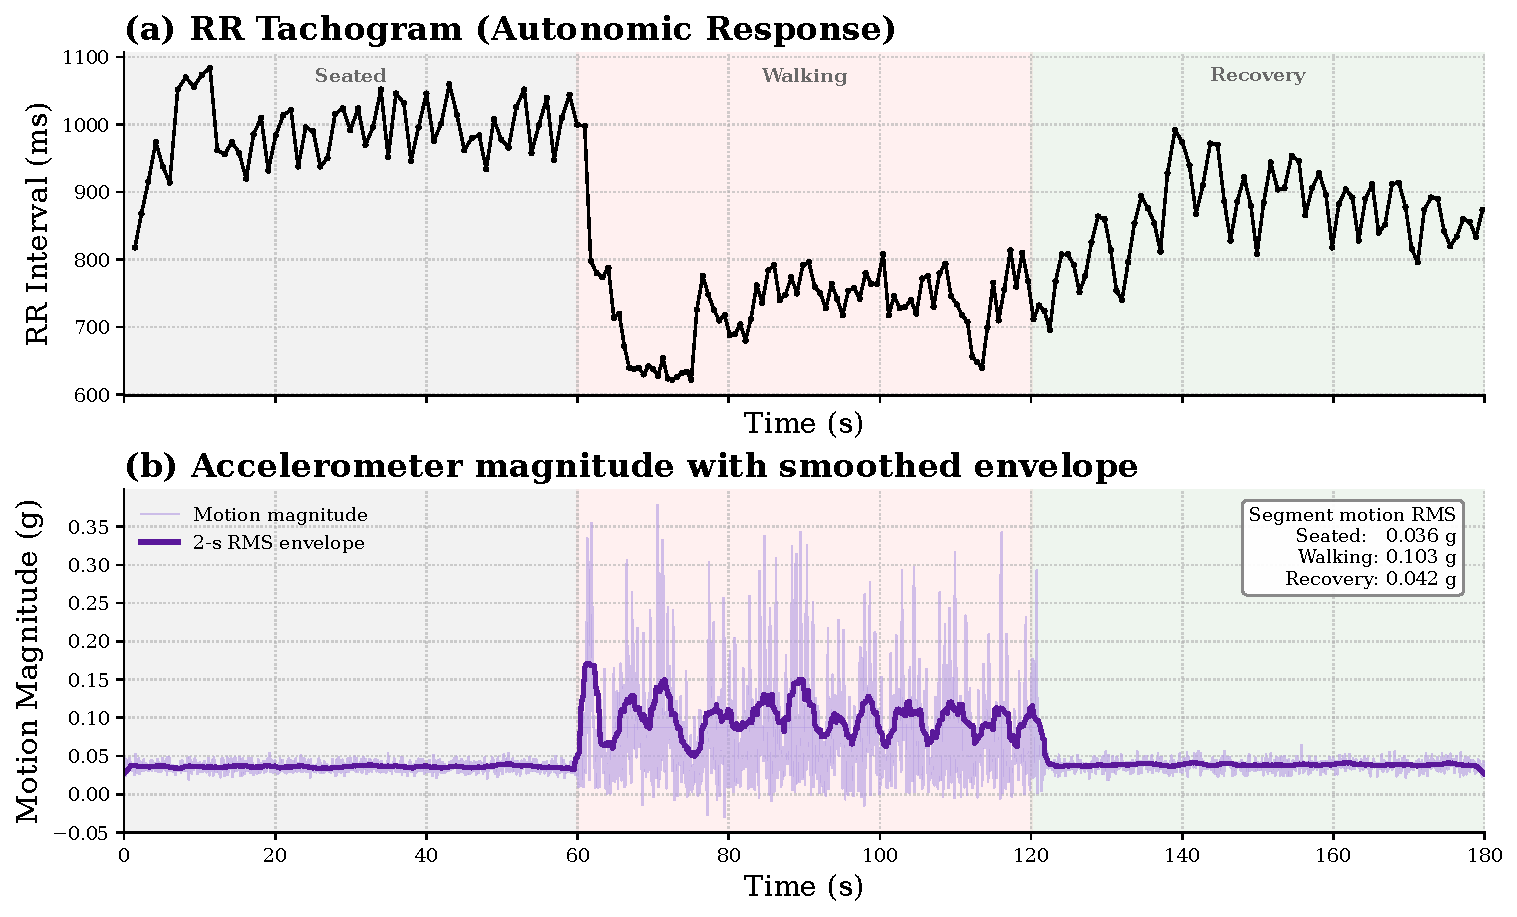
\includegraphics[width=\columnwidth]{nb04_fig05_e3_motion_crosscheck.pdf}
\caption{Walking experiment overview.
(a)~RR tachogram showing the autonomic response across seated,
walking, and recovery segments.  HR rises sharply at walk onset and
decays exponentially during recovery ($\tau = 6.8$~s).
(b)~Accelerometer magnitude with 2-s RMS envelope.  Segment-level
motion RMS confirmed minimal motion during seated (0.036~g) and
recovery (0.042~g), with elevated but moderate motion during walking
(0.103~g).  Time-domain Pearson correlation between
$|\Delta\mathrm{RR}|$ and accelerometer magnitude was $r = 0.26$.}
\label{fig:walk_motion}
\end{figure}

\begin{figure}[!t]
\centering
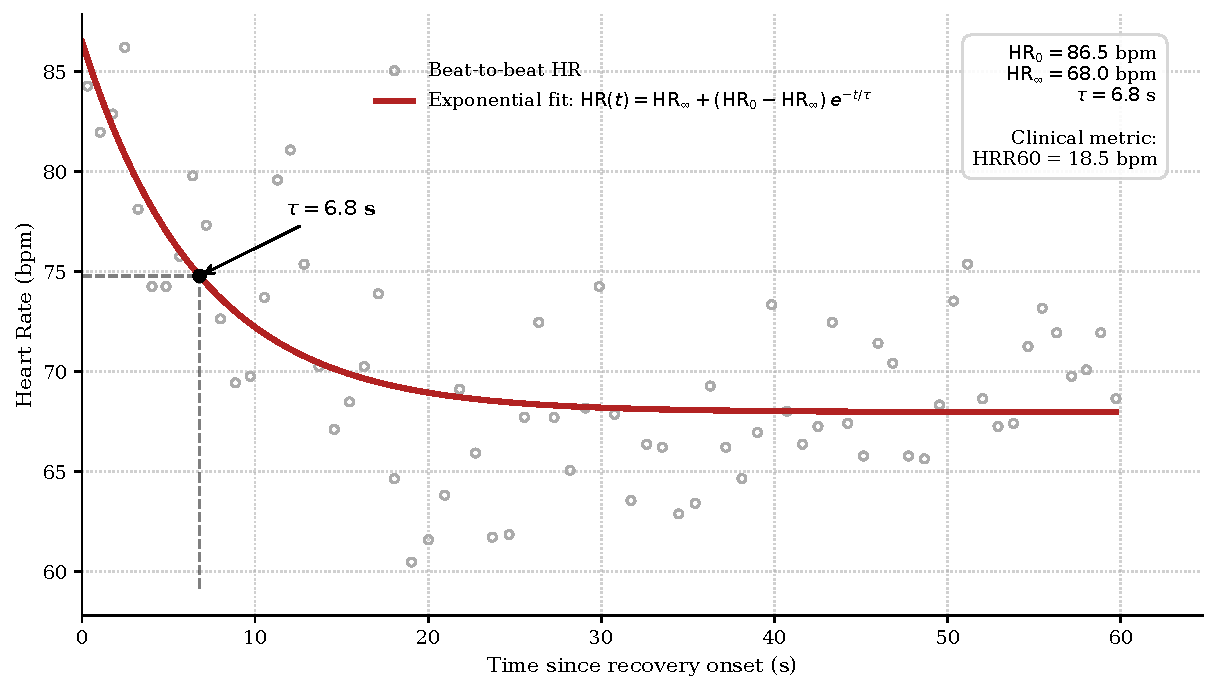
\includegraphics[width=\columnwidth]{nb04_fig03_e3_recovery_tau.pdf}
\caption{Post-walking heart rate recovery fitted to a
single-exponential decay (Eq.~\ref{eq:recovery}).  The time constant
$\tau = 6.8$~s and HRR$_{60} = 18.5$~bpm indicate rapid
parasympathetic reactivation consistent with low-intensity exercise.
Grey circles: beat-to-beat HR; red curve: fitted model
$\mathrm{HR}(t) = A \cdot e^{-t/\tau} + C$.}
\label{fig:recovery_tau}
\end{figure}

\begin{figure}[!t]
\centering
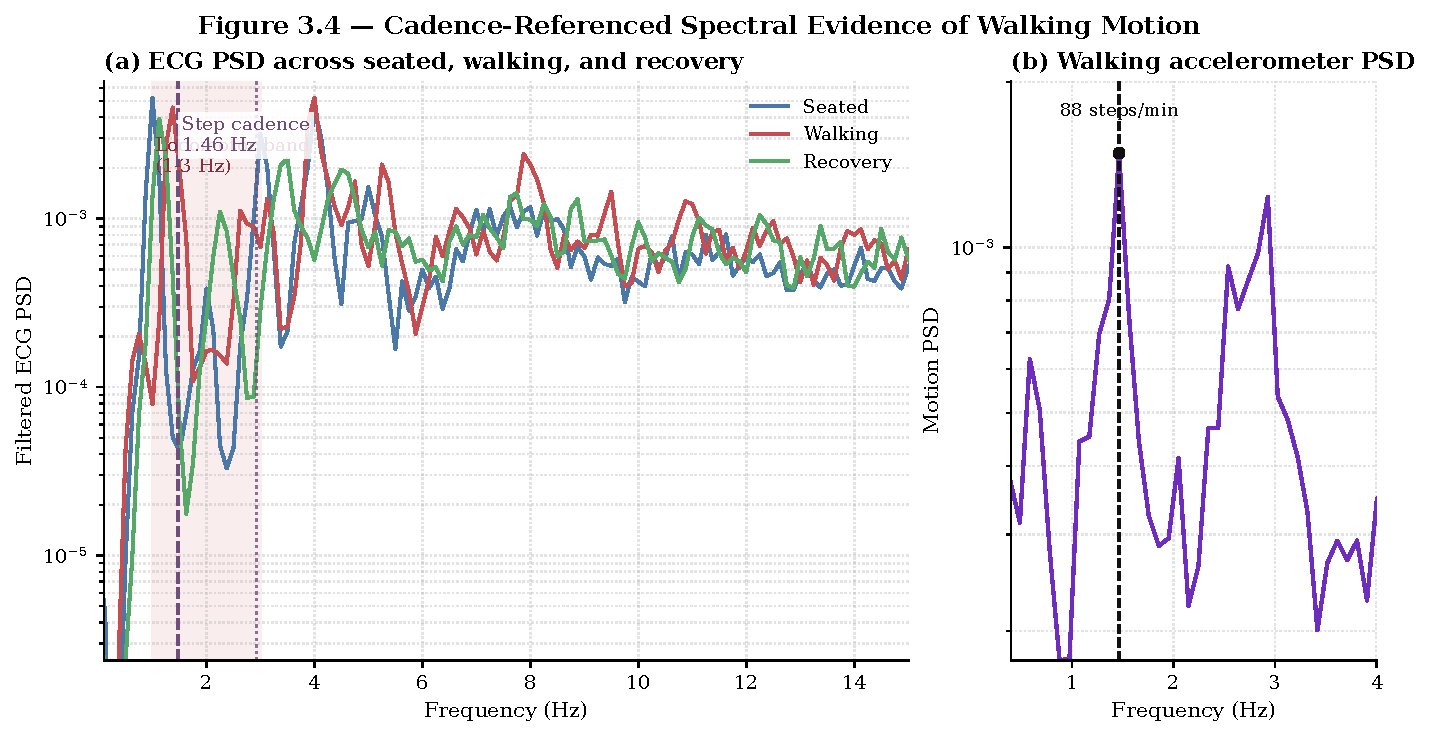
\includegraphics[width=\columnwidth]{nb04_fig04_e3_ecg_psd.pdf}
\caption{Walking-phase ECG power spectral density showing elevated
energy in the 1--3~Hz locomotor band coincident with the walking
cadence.  Motion artifacts contaminate the spectral content during
ambulation, limiting fine-scale HRV interpretation.}
\label{fig:walk_ecg_psd}
\end{figure}



% ------ Paced Breathing ------
\subsection{Paced Breathing: Entrainment Manipulation Check,
LF/HF Band Migration (\textbf{H5}), and Resonance (\textbf{H4})}
\label{ssec:paced}

Experiment~4A was the strongest controlled dose--response component of
this study and yielded three principal findings.

\subsubsection{Frequency Entrainment Was Quantitatively Verified}

The measured RR spectral peak tracked the imposed breathing frequency
with near-perfect fidelity (Fig.~\ref{fig:psd_overlay}).
Linear regression yielded slope~$= 1.022$ (95\% CI: 0.947--1.097),
intercept~$= -0.002$~Hz (95\% CI: $-$0.012 to 0.008),
$R^{2} = 0.998$, and residual SD~$= 0.003$~Hz.
Neither the slope-$=$1 nor the intercept-$=$0 null hypothesis was
rejected, confirming that the manipulation was effective and that the
paced-breathing protocol produced respiratory entrainment of
the cardiac cycle (manipulation check).

\subsubsection{The Primary Effect Was Amplitude Expansion,
Not Heart-Rate Reduction}

Across the five paced conditions, mean HR varied only narrowly
(57.0--60.1~bpm), whereas SDNN rose from 48.7 to 131.4~ms, total
power increased from 1754 to 10{,}493~ms$^{2}$, and peak-to-trough
RR amplitude grew from 157 to 406~ms
(Table~\ref{tab:paced}, Fig.~\ref{fig:e4a_tachograms}).
Slow breathing therefore primarily expanded oscillatory amplitude
rather than shifting the mean chronotropic operating point.

\subsubsection{Respiratory-Centered Spectral Power Did Not Peak at
6~Breaths/Min (\textbf{H4} Supported)}

Classical resonance biofeedback theory predicts a peak in RR
oscillation amplitude near 6~breaths/min
($\sim$0.1~Hz)~\cite{lehrer2014}.
To test this without relying on fixed LF/HF bands or cycle-level
peak-to-trough detection---which can be unstable during very slow
breathing without a direct respiratory belt signal---we computed
respiratory-centered RR spectral power by integrating the Welch PSD
within $\pm$0.015~Hz of each imposed breathing frequency.
Both respiratory-centered power and distribution-based RR amplitude
(p95--p5) increased monotonically from 12~breaths/min to
3~breaths/min (1003 to 13{,}460~ms$^{2}$ and 157 to 406~ms,
respectively; Fig.~\ref{fig:e4a_resp_resonance}), without forming
an inverted-U shape centered at 6~breaths/min.
Sensitivity analysis using $\pm$0.010~Hz and $\pm$0.020~Hz
integration windows confirmed that the absence of an isolated
6-breaths/min peak was robust to the choice of bandwidth
(Appendix, Fig.~\ref{fig:app_sensitivity}).
A classical 6-breaths/min resonance maximum was therefore
\emph{not observed} in this participant under the present
fixed-order protocol (\textbf{H4} supported).

\subsubsection{LF/HF Inflation Dissociated from RMSSD, Supporting
Spectral-Band Migration (\textbf{H5} Supported)}

LF/HF rose dramatically from 0.22 (12/min) to 11.54 (6/min) and
plateaued near 17.5 at the slowest rates, yet RMSSD remained in a
narrow range of 48--66~ms throughout (Fig.~\ref{fig:lfhf_rmssd}).
This dissociation is consistent with \textbf{H5}: when the
respiratory peak crosses the 0.15~Hz LF/HF boundary, the resulting
LF/HF increase reflects respiratory spectral-band migration---not a
genuine sympathovagal reversal~\cite{billman2013}.
RMSSD, being computed entirely in the time domain, is unaffected by
frequency-band assignment and therefore provides a more robust vagal
proxy under slow paced breathing.
Together with the respiratory-centered analysis above, these results
indicate that slow paced breathing inflates LF/HF by mechanically
relocating the dominant respiratory oscillation from HF into LF,
rather than by shifting autonomic balance.


\begin{table}[!t]
\centering
\caption{Paced Breathing: Frequency Tracking and HRV Metrics}
\label{tab:paced}
\footnotesize
\setlength{\tabcolsep}{3.5pt}
\begin{tabular}{@{}lccccc@{}}
\toprule
 & 12/min & 9/min & 6/min & 5/min & 3/min \\
\midrule
Expected (Hz)      & 0.200  & 0.150  & 0.100  & 0.083  & 0.050 \\
Measured (Hz)      & 0.203  & 0.148  & 0.102  & 0.086  & 0.047 \\
$|\Delta f|$ (Hz)  & 0.003  & 0.002  & 0.002  & 0.003  & 0.003 \\
\midrule
HR (bpm)           & 59.4  & 57.0  & 60.2  & 59.9  & 58.1 \\
SDNN (ms)          & 48.7  & 78.0  & 91.3  & 95.9  & 131.4 \\
RMSSD (ms)         & 47.7  & 64.9  & 60.4  & 53.9  & 55.3 \\
TP (ms$^{2}$)      & 1754  & 2381  & 6087  & 8240  & 10{,}493 \\
LF (ms$^{2}$)      & 279   & 953   & 5470  & 7634  & 8980 \\
HF (ms$^{2}$)      & 1242  & 1129  & 474   & 437   & 514 \\
LF/HF              & 0.22  & 0.84  & 11.54 & 17.45 & 17.47 \\
RR amp.\ (ms)      & 157   & 240   & 293   & 297   & 406 \\
\bottomrule
\end{tabular}
\end{table}

\begin{figure}[!t]
\centering
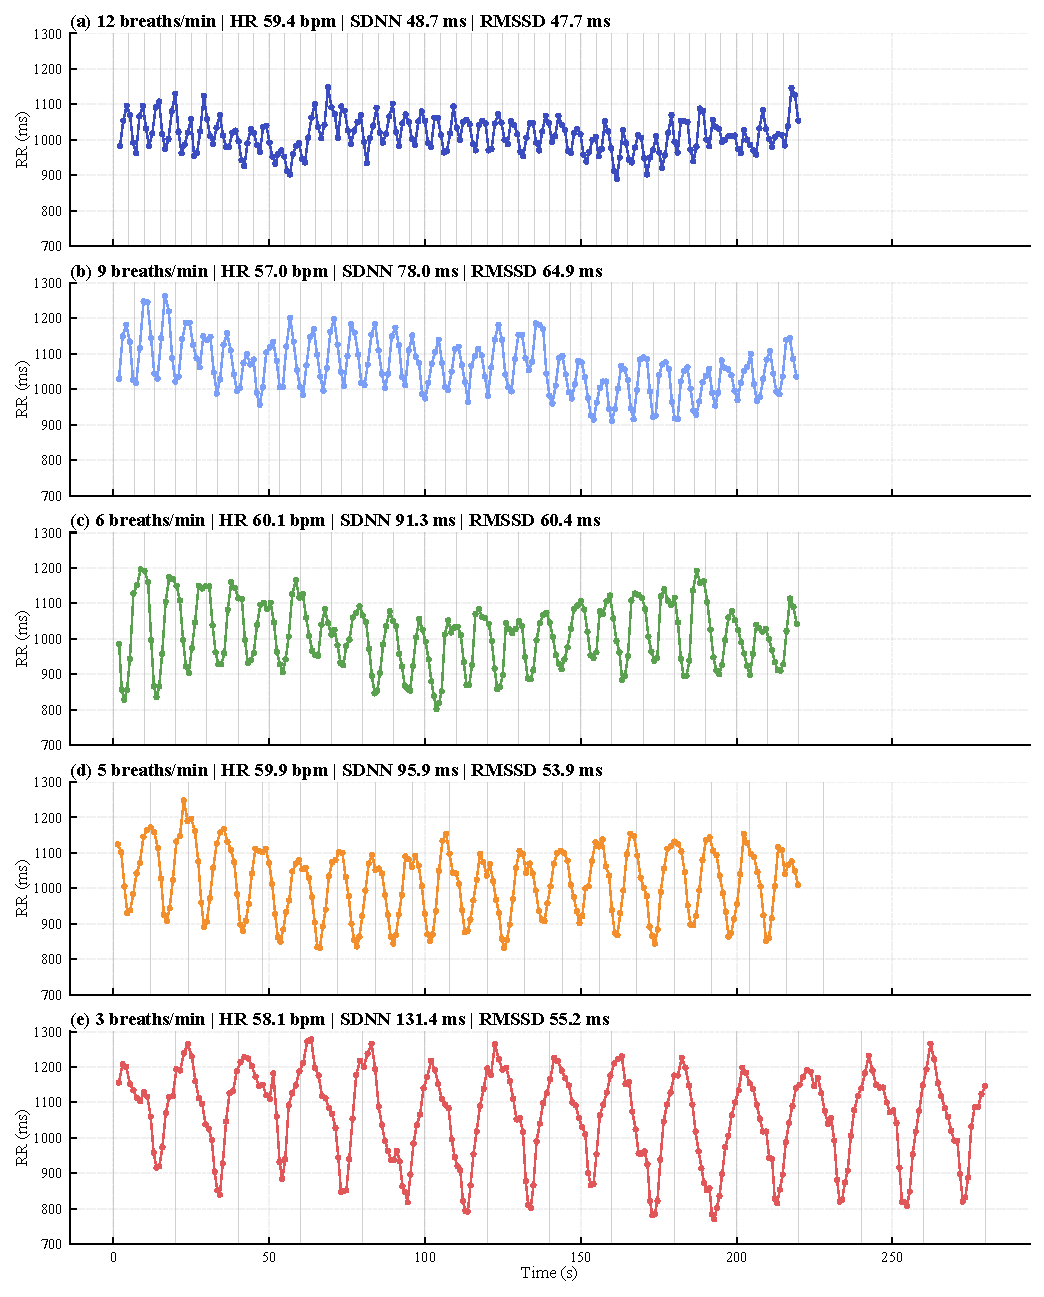
\includegraphics[width=\columnwidth]{nb05_fig01_e4a_tachograms.pdf}
\caption{Paced-breathing RR tachograms for five breathing rates (12,
9, 6, 5, 3~breaths/min).  Light grey vertical lines indicate
metronome-cued inhalation onsets used by the participant to pace
breathing.  RR oscillation amplitude increases progressively with
slower breathing, while mean RR interval (and thus HR) remains
relatively stable across conditions.}
\label{fig:e4a_tachograms}
\end{figure}

\begin{figure}[!t]
\centering
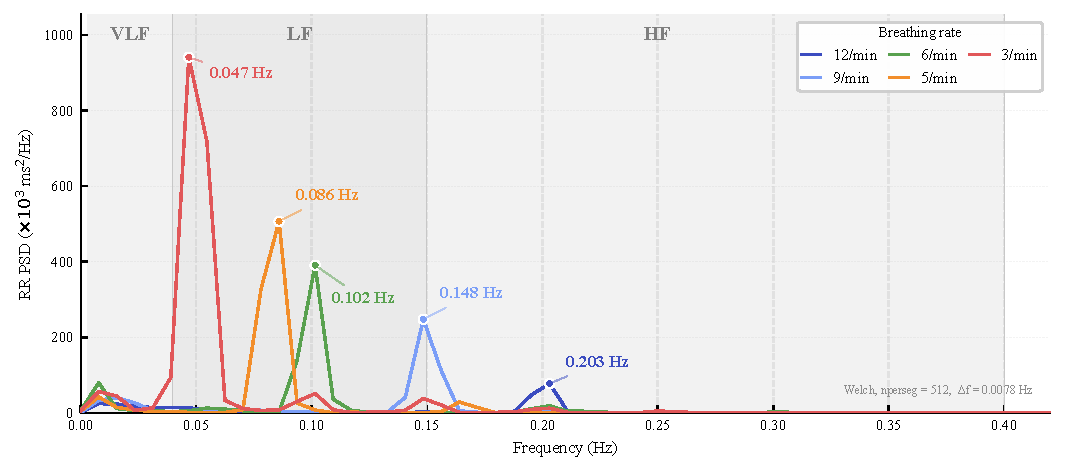
\includegraphics[width=\columnwidth]{nb05_fig02_e4a_psd_overlay.pdf}
\caption{RR interval PSD for five paced-breathing conditions.
The dominant spectral peak migrates leftward with decreasing
breathing rate, crossing the LF/HF boundary (dashed vertical line
at 0.15~Hz) between 12/min and 6/min.  Peak amplitude increases
monotonically with slower breathing.}
\label{fig:psd_overlay}
\end{figure}

\begin{figure}[!t]
\centering
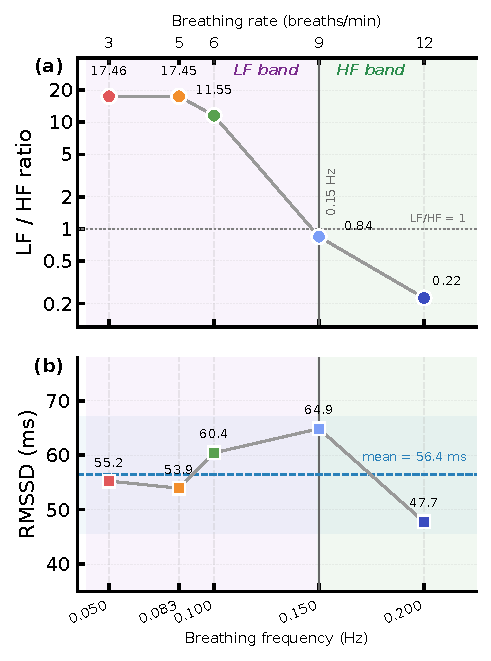
\includegraphics[width=\columnwidth]{nb05_fig04_e4a_lfhf_crossover.pdf}
\caption{LF/HF ratio (left axis) vs.\ RMSSD (right axis) across
paced-breathing conditions.  LF/HF inflates dramatically below
9~breaths/min while RMSSD remains stable, demonstrating that the
LF/HF increase reflects spectral-band migration rather than
sympathovagal reversal.}
\label{fig:lfhf_rmssd}
\end{figure}

\begin{figure}[!t]
\centering
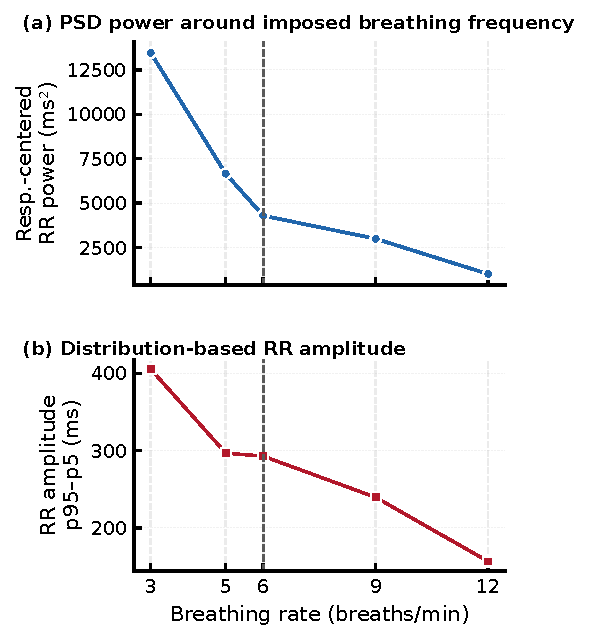
\includegraphics[width=\columnwidth]{nb05_fig05b_e4a_resp_power_and_amplitude.pdf}
\caption{Resonance assessment via respiratory-centered metrics.
(a)~RR PSD power integrated within $\pm$0.015~Hz of each imposed
breathing frequency.
(b)~Distribution-based RR amplitude (p95--p5).
Both measures increase monotonically from 12 to 3~breaths/min;
neither exhibits an inverted-U maximum at 6~breaths/min (dashed
vertical line).
A classical 6-breaths/min resonance peak was not observed in this
participant under the present fixed-order protocol.}
\label{fig:e4a_resp_resonance}
\end{figure}


% ------ Cross-Experiment ------
\subsection{Cross-Experiment Synthesis Required
Task-Specific Summary Spaces}
\label{ssec:integration}

When all experiments are viewed together
(Fig.~\ref{fig:integration}), two distinct physiological axes emerge.
\emph{Posture} primarily shifted the autonomic operating point along
a trajectory of increasing HR and decreasing RMSSD (supine
$\to$ standing), with total power declining monotonically.
\emph{Paced breathing}, by contrast, maintained nearly stable
mean~HR while expanding total power by a factor of 6.0
(1754$\to$10{,}493~ms$^{2}$) and SDNN by a factor of 2.7.

These are fundamentally different types of physiological modulation
and cannot be ranked on a single LF/HF axis.
The breath-hold and walking paradigms, meanwhile, are best described
as challenge--recovery trajectories: inspiratory hold showed the
stronger HR rise, expiratory recovery showed the largest RMSSD
rebound, and walking recovery followed an exponential time course.

We therefore advocate reporting cross-experiment summaries using
mean~HR, RMSSD, total power, and explicit validity annotations
(e.g., ``motion-limited,'' ``band-shifted'') rather than forcing
all conditions into a single frequency-domain scalar.

\begin{figure}[!t]
\centering
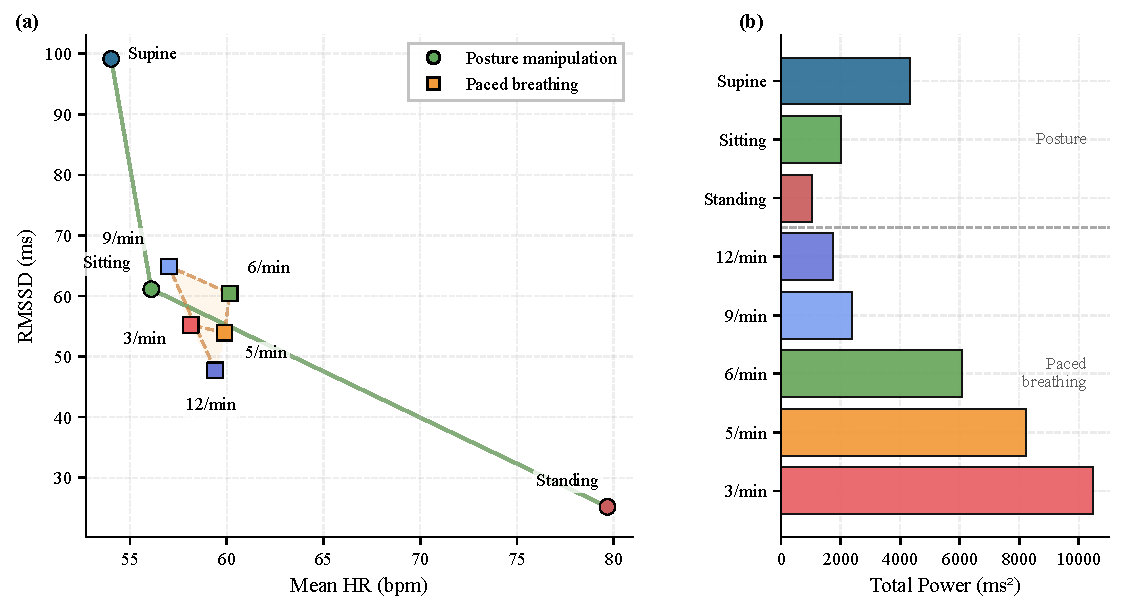
\includegraphics[width=\columnwidth]{nb06_fig01_autonomic_spectrum.pdf}
\caption{Cross-experiment autonomic map.  Steady-state conditions
are plotted by LF and HF power (log scale) with mean HR on a
twin axis.  Posture shifts the operating point along the HR axis;
paced breathing expands total spectral power at nearly constant HR.
Transient experiments (breath-hold, walking) appear in separate
annotations.}
\label{fig:integration}
\end{figure}


% ============================================================
\section{Discussion}
\label{sec:discussion}

\subsection{Context Determines Interpretation}

The central finding of this study is that HRV indices do not have
context-free meaning.
The same LF/HF ratio that meaningfully distinguished supine from
standing (0.28 vs.\ 1.44) became physiologically uninterpretable
under slow paced breathing (17.47), where it was driven entirely
by the mechanical relocation of the respiratory peak from HF into
LF.
This result aligns with longstanding critiques that LF/HF ``does not
accurately measure cardiac sympatho-vagal
balance''~\cite{billman2013,eckberg1997} and extends them by
providing direct within-subject evidence: the same participant
generated a 60-fold range in LF/HF (0.28--17.47) through postural
and respiratory manipulations alone, without any pharmacological or
pathological intervention.

\subsection{Paced Breathing: Amplitude, Not Rate}

An underappreciated aspect of slow-breathing effects is that the
primary physiological change is amplitude expansion of the
respiratory sinus arrhythmia, not reduction of mean heart rate.
In our data, mean HR varied by only 3.1~bpm across the five paced
conditions (57.0--60.1~bpm), whereas peak-to-trough RR amplitude
increased by 159\% (157--406~ms).
This finding is consistent with the view that slow breathing
amplifies the gain of the cardiorespiratory coupling
loop---the baroreflex, respiratory gating of vagal
efferents~\cite{hirsch1981}, and mechanical intrathoracic pressure
oscillations---without substantially altering the mean autonomic
tone~\cite{berntson1997,penttila2001}.

The absence of a 6-breaths/min resonance maximum in this participant
warrants cautious interpretation.
Classical resonance theory~\cite{lehrer2014} predicts that RR
oscillation amplitude peaks when breathing frequency matches the
cardiovascular system's natural resonance, typically near 0.1~Hz.
Using respiratory-centered RR spectral power---a metric that
tracks the imposed breathing frequency rather than relying on fixed
LF/HF bands---we found that both spectral power and RR amplitude
(p95--p5) increased monotonically down to 3~breaths/min (0.05~Hz).
This pattern was robust across three integration bandwidths
($\pm$0.010, $\pm$0.015, $\pm$0.020~Hz).
However, this is a single-participant observation under a
fixed descending presentation order (12$\to$3~breaths/min), so the
monotonic increase may partly reflect progressive relaxation, deeper
tidal volumes at slower rates, or cumulative training effects
rather than a genuine absence of resonance.
A randomized or counterbalanced multi-participant design with
concurrent respiratory monitoring would be needed to distinguish
these possibilities from a true resonance-frequency shift.

\subsection{Practical Implications for HRV Reporting}

Based on these findings, we suggest three practical guidelines
for HRV reporting in multi-paradigm studies:
\begin{enumerate}
\item Report LF/HF only when breathing rate is confirmed to lie
  within the HF band ($>$0.15~Hz, i.e., $>$9~breaths/min).
  Otherwise, use RMSSD or total power as the primary summary.
\item Annotate each condition with a validity note indicating
  whether the standard interpretive framework applies (e.g.,
  ``standard,'' ``band-shifted,'' ``motion-limited'').
\item Use posture-matched anchors when comparing transient tasks
  against baselines, to avoid confounding postural and
  task-specific autonomic effects.
\end{enumerate}

Table~\ref{tab:validity} consolidates the task-specific validity of
standard HRV metrics observed across all four experiments, providing
a practical reference for interpreting HRV under each tested
condition.

\begin{table}[!t]
\caption{Task-Specific HRV Metric Validity Summary}
\label{tab:validity}
\centering
\footnotesize
\begin{tabular}{@{}p{2.2cm}p{1.5cm}p{2.1cm}p{2.7cm}@{}}
\toprule
Condition & HRV valid? & Primary metric & Caveat \\
\midrule
Supine/sitting/\newline standing (E1) & Yes & RMSSD, HF, LF/HF & Steady-state \\
\addlinespace
Breath-hold (E2) & Partial & HR response, recovery, HF & Transient; short-segment PSD \\
\addlinespace
Walking (E3) & Motion-limited & Mean HR, recovery $\tau$ & RMSSD unreliable \\
\addlinespace
Paced $\geq$9/min (E4) & Mostly valid & RMSSD, HF, LF/HF & Resp.\ peak in or near HF band \\
\addlinespace
Paced $\leq$6/min (E4) & Band-shifted & RMSSD, total power, RR ampl., resp.-centered power & LF/HF invalid as sympathovagal index; use resp.-centered power for resonance \\
\bottomrule
\end{tabular}
\end{table}


% ============================================================
\section{Limitations}
\label{sec:limitations}

This lab study has five principal limitations.
First, it is a single-participant within-subject investigation; the
findings illustrate metric-behavior principles under controlled
within-subject manipulation but cannot claim population
generalizability.
We deliberately framed this as a methodological lab demonstration
rather than an inferential study.

Second, the paced-breathing conditions were presented in fixed
descending order (12$\to$3~breaths/min), so progressive relaxation,
training, or fatigue effects cannot be fully separated from the
breathing-rate manipulation.

Third, no direct respiratory signal (respiratory belt or impedance
pneumography) was recorded.
Respiratory entrainment was inferred from the RR spectral peak;
ECG-derived respiration (EDR) validation is recommended for future
iterations of this lab.

Fourth, walking-phase HRV is motion-contaminated, and fine-scale
beat-to-beat metrics during ambulation should be interpreted with
explicit motion-limited validity caveats.
Magnitude-squared coherence between the walking ECG and accelerometer
was low ($C_{xy} = 0.04$ at the step peak), consistent with absence of
strong phase-locked linear coupling but not excluding broadband or
non-linear artifact; the combination of high accelerometer motion and
cadence-proximate spectral energy warrants caution for fine-scale HRV
indices.

Despite these limitations, the within-subject design provides a
controlled demonstration of context-dependent HRV metric behavior
across four physiologically distinct paradigms.


% ============================================================
\section{Conclusion}
\label{sec:conclusion}

Using a unified single-lead ECG pipeline across four
assignment-specified paradigms, this lab study showed that different
physiological tasks modulate different aspects of cardiorespiratory
regulation.
Posture shifts the autonomic operating point (\textbf{H1}).
Breath-hold reveals asymmetric inspiratory--expiratory dynamics
(\textbf{H2}).
Walking produces genuine cardiovascular load but limits fine-scale
HRV interpretability (\textbf{H3}).
Within the tested range of paced breathing, no classical
6-breaths/min resonance maximum was observed (\textbf{H4}).
Slow paced breathing exposes LF/HF as a band-migration artifact
rather than a sympathovagal index (\textbf{H5}).
The most important methodological conclusion, summarized in the
validity table (Table~\ref{tab:validity}), is that HRV metrics
cannot be interpreted independently of the physiological context.
Under slow paced breathing, mean~HR, RMSSD, and total
power---not LF/HF---provide the most robust cross-condition summary.


% ============================================================
% REFERENCES
% ============================================================
\begin{thebibliography}{99}

\bibitem{taskforce1996}
Task Force of the European Society of Cardiology and the North
American Society of Pacing and Electrophysiology,
``Heart rate variability: Standards of measurement, physiological
interpretation, and clinical use,''
\emph{Circulation}, vol.~93, no.~5, pp.~1043--1065, 1996.

\bibitem{pan1985}
J.~Pan and W.~J.~Tompkins,
``A real-time QRS detection algorithm,''
\emph{IEEE Trans.\ Biomed.\ Eng.}, vol.~BME-32, no.~3,
pp.~230--236, Mar.~1985.

\bibitem{berntson1997}
G.~G.~Berntson \emph{et~al.},
``Heart rate variability: Origins, methods, and interpretive
caveats,''
\emph{Psychophysiology}, vol.~34, no.~6, pp.~623--648, 1997.

\bibitem{billman2013}
G.~E.~Billman,
``The LF/HF ratio does not accurately measure cardiac
sympatho-vagal balance,''
\emph{Front.\ Physiol.}, vol.~4, article~26, 2013.

\bibitem{shaffer2017}
F.~Shaffer and J.~P.~Ginsberg,
``An overview of heart rate variability metrics and norms,''
\emph{Front.\ Public Health}, vol.~5, article~258, 2017.

\bibitem{lehrer2014}
P.~M.~Lehrer and R.~Gevirtz,
``Heart rate variability biofeedback: How and why does it work?''
\emph{Front.\ Psychol.}, vol.~5, article~756, 2014.

\bibitem{makowski2021}
D.~Makowski \emph{et~al.},
``NeuroKit2: A Python toolbox for neurophysiological signal
processing,''
\emph{Behav.\ Res.\ Methods}, vol.~53, no.~4, pp.~1689--1696,
2021.

\bibitem{virtanen2020}
P.~Virtanen \emph{et~al.},
``SciPy 1.0: Fundamental algorithms for scientific computing in
Python,''
\emph{Nature Methods}, vol.~17, no.~3, pp.~261--272, 2020.

\bibitem{eckberg1997}
D.~L.~Eckberg,
``Sympathovagal balance: A critical appraisal,''
\emph{Circulation}, vol.~96, no.~9, pp.~3224--3232, 1997.

\bibitem{hirsch1981}
J.~A.~Hirsch and B.~Bishop,
``Respiratory sinus arrhythmia in humans: How breathing pattern
modulates heart rate,''
\emph{Am.\ J.\ Physiol.}, vol.~241, no.~4, pp.~H620--H629, 1981.

\bibitem{penttila2001}
J.~Penttil\"a, A.~Helminen, T.~Jartti, \emph{et~al.},
``Time domain, geometrical and frequency domain analysis of cardiac
vagal outflow: Effects of various respiratory patterns,''
\emph{Clin.\ Physiol.}, vol.~21, no.~3, pp.~365--376, 2001.

\end{thebibliography}

% ============================================================
% APPENDICES
% ============================================================
\appendices

\section{Data Quality and Pipeline Validation}
\label{app:quality}

Dual-path R-peak detection (SciPy teaching path vs.\ NeuroKit2
reference path) was validated on the E1A 5-min supine recording.
Peak count agreement was 99.6\% (269 vs.\ 268 peaks).
The mean RR difference was 0.96~ms (0.09\%), SDNN difference was
1.65~ms (2.1\%), and RMSSD difference was 2.69~ms (2.7\%).
Across all 8~steady-state sessions, peak-count agreement
exceeded 99.5\%.

\begin{figure}[!t]
\centering
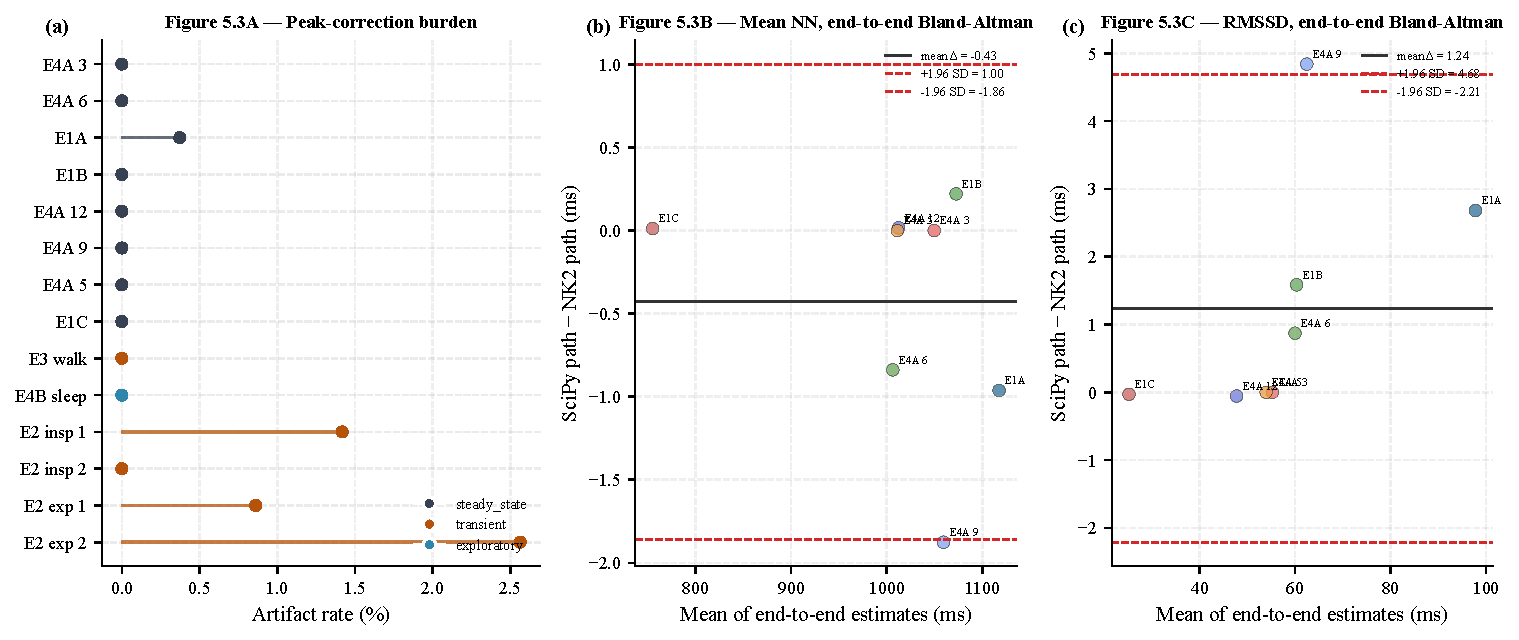
\includegraphics[width=\columnwidth]{nb06_fig03_pipeline_validation.pdf}
\caption{Pipeline validation across all steady-state recordings:
artifact rate and dual-path agreement metrics.}
\label{fig:app_pipeline}
\end{figure}



\section{Postural Detail Figures}
\label{app:posture_detail}

\begin{figure}[!t]
\centering
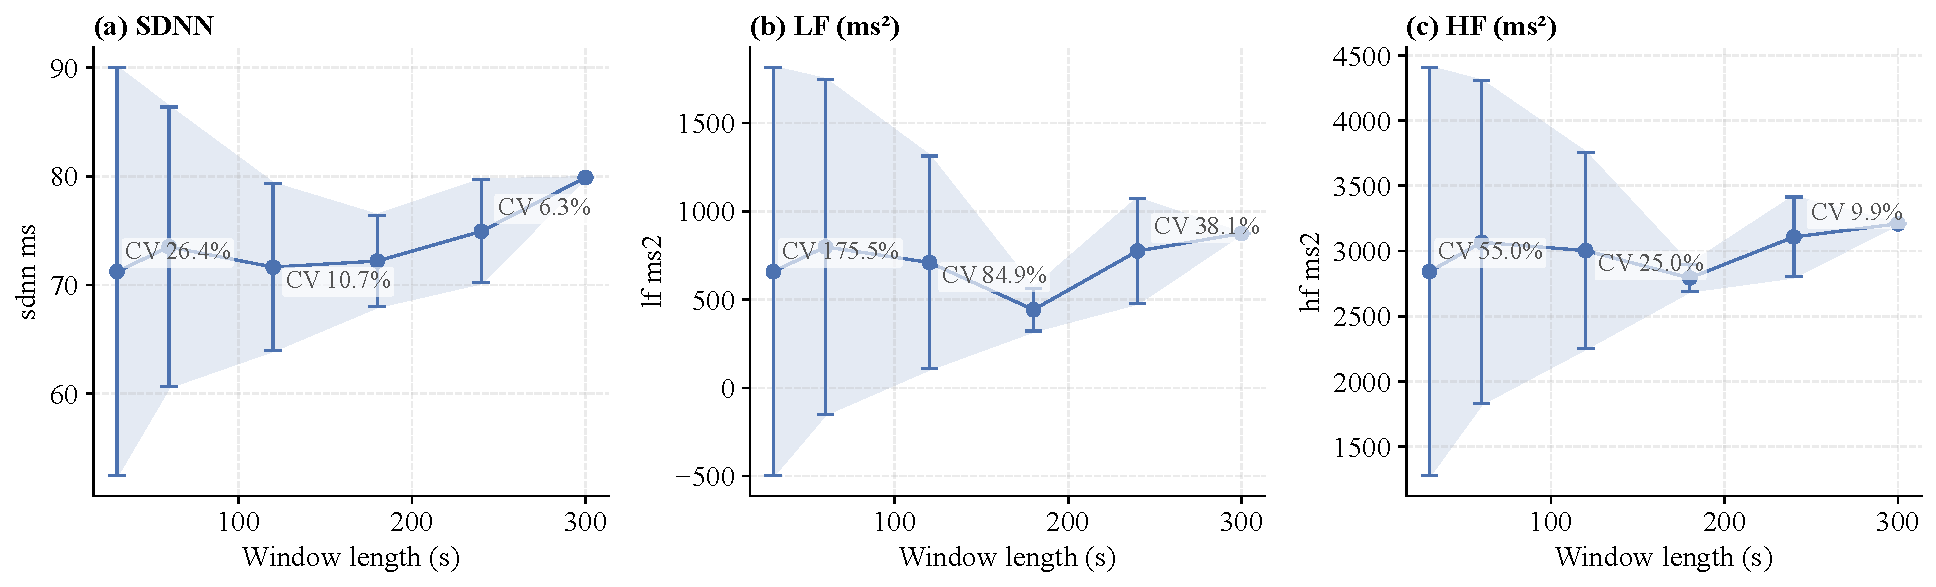
\includegraphics[width=\columnwidth]{nb02_fig04_duration_effect.pdf}
\caption{Effect of analysis window duration on HRV metric stability
across postural conditions.}
\label{fig:app_duration}
\end{figure}


\section{Breath-Hold Trial-Level Detail}
\label{app:breathhold_detail}

\begin{figure}[!t]
\centering
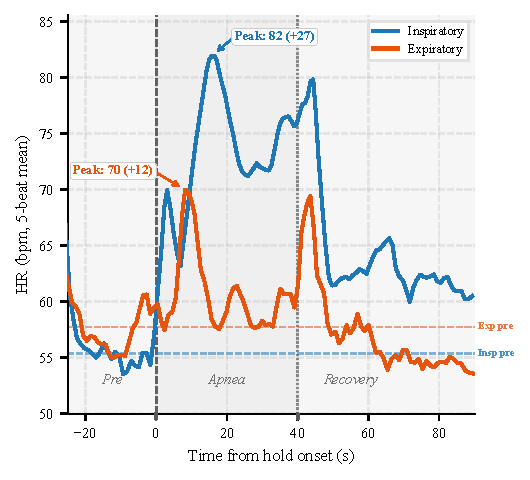
\includegraphics[width=\columnwidth]{nb03_fig03_e2_pure_physiology.pdf}
\caption{Trial-level breath-hold physiological responses, showing
individual HR trajectories for each inspiratory and expiratory
trial.}
\label{fig:app_pure_physiology}
\end{figure}


\section{Walking Detail Figures}
\label{app:walking_detail}

\begin{figure}[!t]
\centering
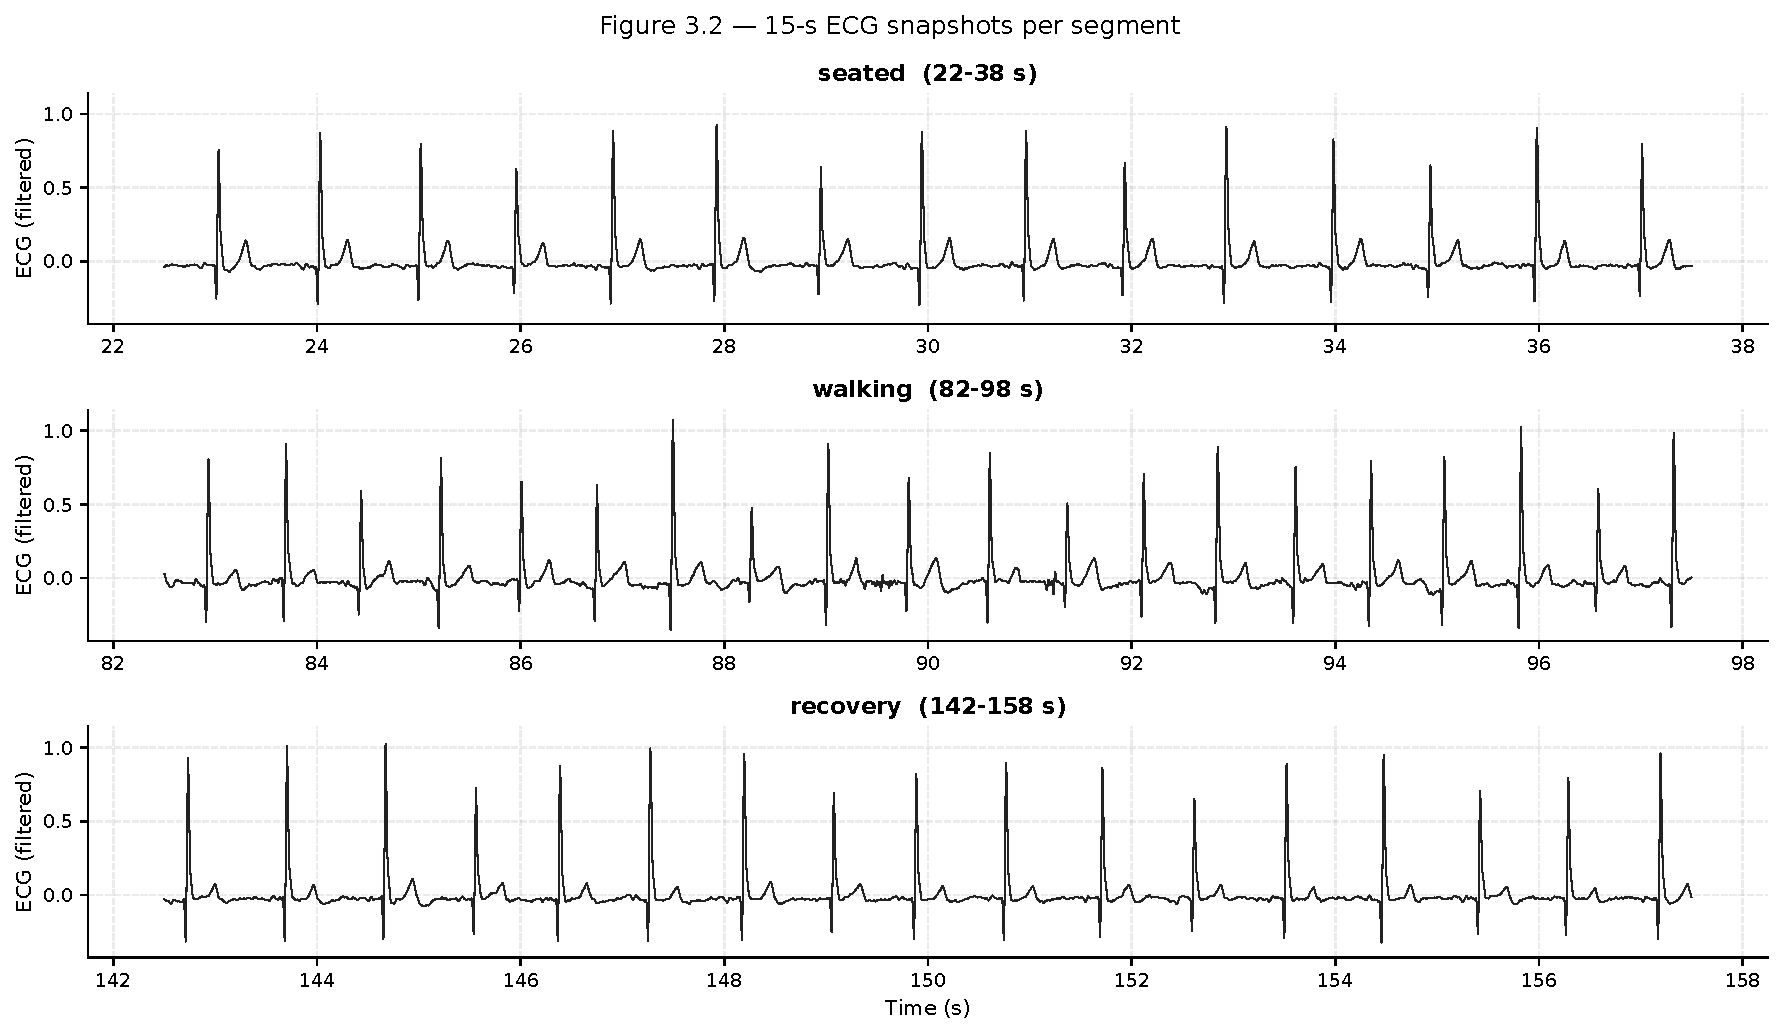
\includegraphics[width=\columnwidth]{nb04_fig02_e3_ecg_snapshots.pdf}
\caption{ECG signal processing during the walking segment (60--70~s).
(a)~Raw ECG showing motion artifacts and baseline wander
characteristic of ambulatory recording.
(b)~Bandpass-filtered signal with substantially reduced
low-frequency drift.
(c)~R-peak detection on the filtered signal.  Despite visible motion
contamination, the NeuroKit2 detector successfully identified all QRS
complexes in this segment.}
\label{fig:app_ecg_snapshots}
\end{figure}

\begin{figure}[!t]
\centering
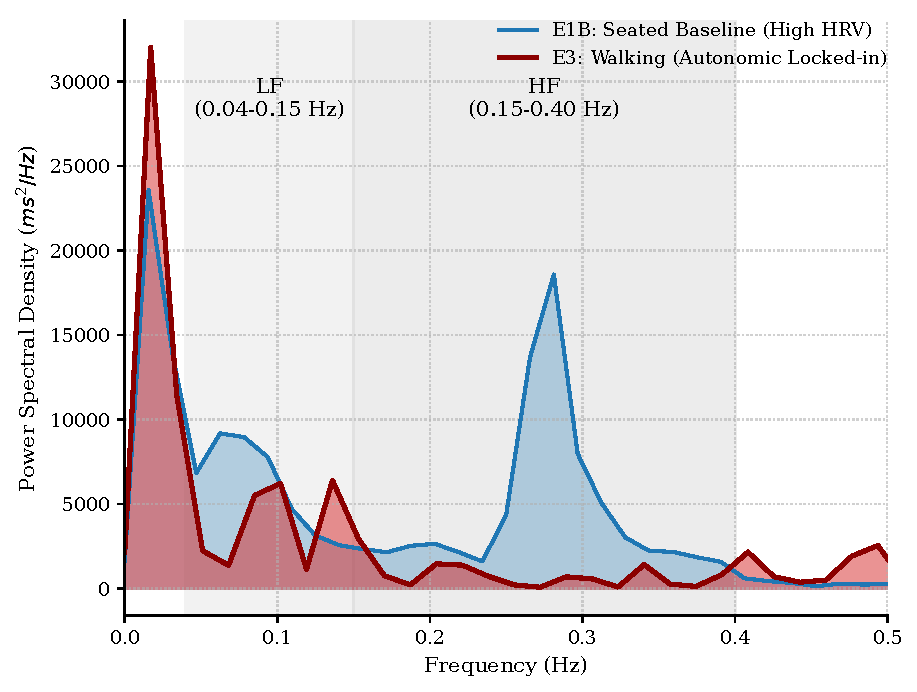
\includegraphics[width=\columnwidth]{nb04_fig06_e3_rr_psd_contrast.pdf}
\caption{Walking vs.\ recovery RR power spectral density contrast.}
\label{fig:app_rr_psd_contrast}
\end{figure}

\section{Paced Breathing Resonance: Sensitivity Analysis}
\label{app:resonance}

\begin{figure}[!t]
\centering
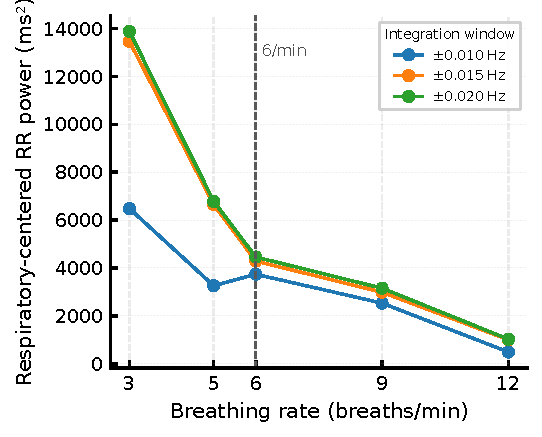
\includegraphics[width=\columnwidth]{nb05_fig05_e4a_resp_centered_power.pdf}
\caption{Sensitivity analysis of respiratory-centered RR spectral
power across three integration windows ($\pm$0.010, $\pm$0.015,
$\pm$0.020~Hz) around each imposed breathing frequency.
Across all three bandwidths, power increases monotonically from
12 to 3~breaths/min; no isolated peak appears at 6~breaths/min
(dashed vertical line).
The consistency across bandwidths indicates that the absence of a
classical 6-breaths/min resonance maximum is not an artifact of
integration-window choice.}
\label{fig:app_sensitivity}
\end{figure}

\balance
\end{document}
